\begin{savequote}[75mm] 
Live long and prosper
\qauthor{Spock} 
\end{savequote}

\chapter{Machine learning based algorithm for long-lived particles reconstruction in LHCb}
\label{chapter:PLLT}

This chapter presents a Machine Learning based study related to the improvement of the Downstream Tracking algorithm. It starts by providing the general introduction to the LHCb track reconstruction methodology, and the Downstream Tracking algorithm is described, including a section focused on a seed classifier. Then, the performance of the entire Downstream Tracking algorithm is discussed. The final section is dedicated to present ideas on how to approach similar types of problems by leveraging more sophisticated Deep Learning models. Those models will be tested as a part of the development of the Downstream Tracking algorithm for the Upgraded LHCb experiment.   

\section{Track reconstruction}
Tracking is one of the essential steps in event reconstruction. This procedure is dedicated to reconstructing particle trajectories using a collection of hits that were created when a particle interacts with tracking stations. Tracks are used to provide precision vertexing and momentum estimation. Without that information, no physics analysis can be performed. Moreover, track information together is important is crucial for particle identification. Calorimeter cluster, muon station hits, and Cherenkov rings need associated tracks to be properly reconstructed.

The tracking procedure consists of three major subroutines listed below: 

\begin{itemize}
    \item \textbf{Pattern Recognition}. Pattern recognition is the first step in the tracking reconstruction sequence, that is responsible for associating hits to a given particle. These algorithms have to deal with big combinatorics, which originates from the number of hits that are recorded by the tracking detectors. 

    The pattern recognition efficiency has vital importance. In order to reconstruct $B$ meson decays, one has to reconstruct several tracks. As an example, let consider decay channel $B^0 \rightarrow K^{*0} (\rightarrow K^+\pi^âˆ')\mu^+  + \mu^âˆ' $, which is one of the most promising channels to detect a New Physics phenomena \cite{k*mumu}. In this case, in order to accurately reconstruct $B^0$, meson four charged particles have to be reconstructed. Thus the efficiency of $B$ meson reconstruction depends on the fourth-order on the track reconstruction efficiency. 
    Pattern recognition algorithms have to be fast. Thus there are executed as a part of software online trigger, for which timing is essential. 
\item \textbf{Track Fitting}. The tracks that were found by the pattern reconstruction are then fitted using a Kalman filter approach \cite{kalman}\cite{kalman2}. This method is capable of accounting multiple scattering and energy loss in the detector. This tracking reconstruction subroutine is the most CPU time consuming because it has to perform the intense computation of material interaction and propagation through the magnetic field. The detailed description of how this method is utilized within the LHCb tracking can  be found in   

\item \textbf{Clone killing}. The final step in the Track reconstruction is called Clone killing. In this stage, tracks that have been reconstructed multiple times are eliminated. Those duplicated tracks originate from the redundant pattern recognition when the algorithms create two tracks with similar hits content. The outcome of this step can be used for physics analysis.   
\end{itemize}



\section{The LHCb track types}
The tracks reconstructed in the LHCb detector are split into five categories. The splitting criterion is based on subdetectors in which they were reconstructed, which is shown in figure \ref{fig:track_types}. 


\begin{figure}
\centering
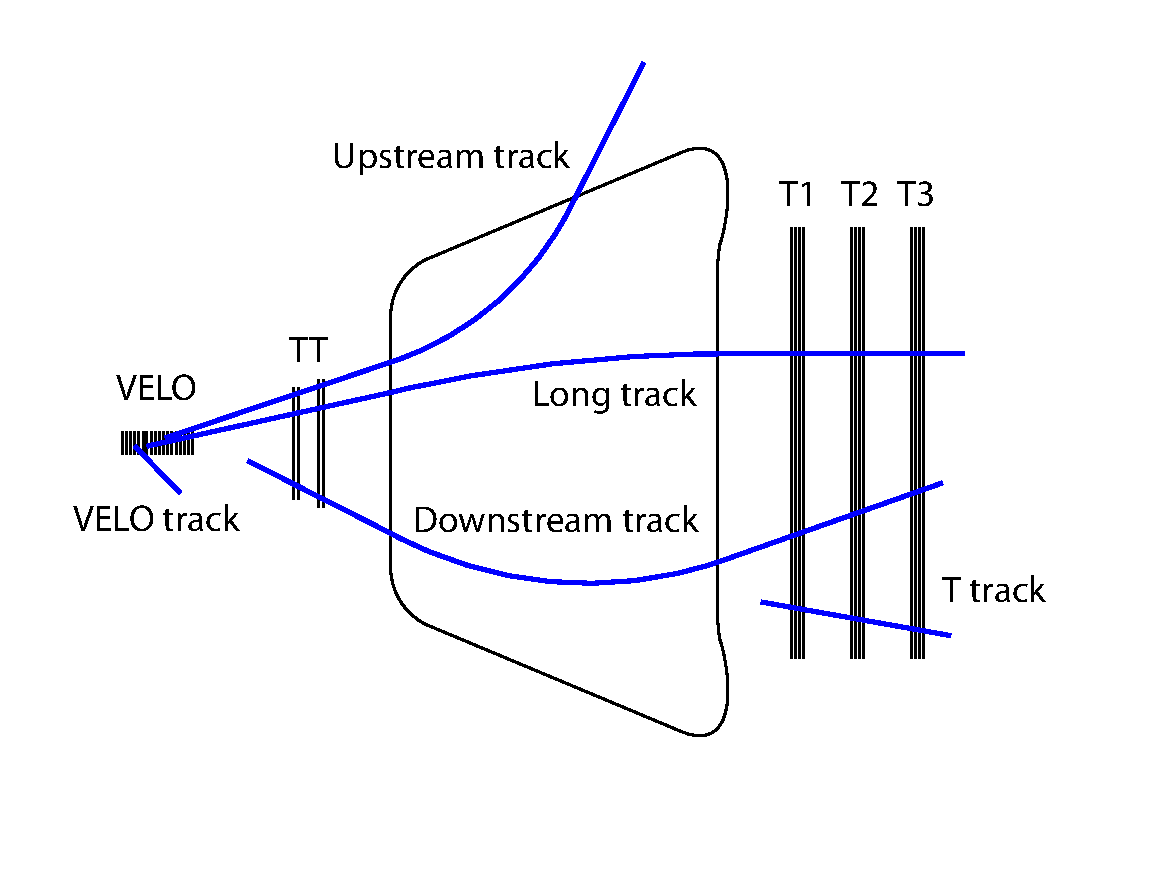
\includegraphics[scale=0.9]{figures/trackTypes.pdf}
\caption{Track types available in the LHCb and corresponding subdetectors. 
\label{fig:track_types}}
\end{figure}

The first category of the tracks is \textbf{VELO tracks}. That tracks are reconstructed using only hits measured in the VELO detector. Therefore, for this track, momentum measurement is impossible. Nevertheless, VELO tracks also play an essential role in classifiers designed to select isolated particles, for instance, when the analysis focuses on searching for rare or forbidden decays. 

The second type of track is \textbf{Upstream tracks}. They consist of VELO segments matched with hits in the TT detector. This track is reconstructed to expand the detector's acceptance for low momentum particles, which would otherwise be removed by the magnet. However, because of the weak residual magnetic field in TT, the estimated momentum resolution for these tracks is worst than 10\%.

\textbf{T tracks} are defined as those which have measurements only in T stations. Despite the worst momentum resolution, around 25\%, they play a vital role in improving the purity of LHCB's photon reconstruction by identifying Electromagnetic Calorimeter clusters create by the electrons. 

The most important category is \textbf{Long tracks}, which contains those tracks which originate
in the vertex detector and traverse the full tracker acceptance, including passing through T and TT stations. These tracks provide the best momentum resolution for particles that traverse the full tracking detector and are used in the majority of LHCb analyses.

The final most significant from this thesis perspective, a group of tracks, are \textbf{Downstream tracks}. The Downstream track contains T-segments matched to the hits in the TT. Those tracks are created by the daughters of the long-lived particles, which decays outside of the VELO detector. The reconstruction of the Downstream tracks allows almost double the LHCb acceptance for long-lived particles. Those tracks are reconstructed by the PatLongLivedTracking algorithm. 
The accurate description of this algorithm is a topic of section \ref{Sec:Downstrean Overview}. 

Within the framework of LHCb experiment, a track is modelled as a series of straight line segments, known as track states. A track state is defined as a 5 dimensional vector of the form:
\begin{equation}
    \vec{x} = \begin{pmatrix}
    x \\ y \\ t_{x} \\ t_{y} \\ \frac{p}{q} 
    \end{pmatrix}
\end{equation}

where: $t_x = \frac{\partial x}{\partial z}$ and $t_y = \frac{\partial y}{\partial z}$, $p$ is a track momentum and $q$ is a track's associated particle charge. It is worth to notice that LHCb uses the coordinate system, which is right-handed. The $x-z$ is bending plane and the $y-z$ is non-bending. 


To visualize the complexity of tracking reconstruction problem figure \ref{fig:event display} presents a single event display, that was collected during Run II.   




\begin{figure}[h]
\centering
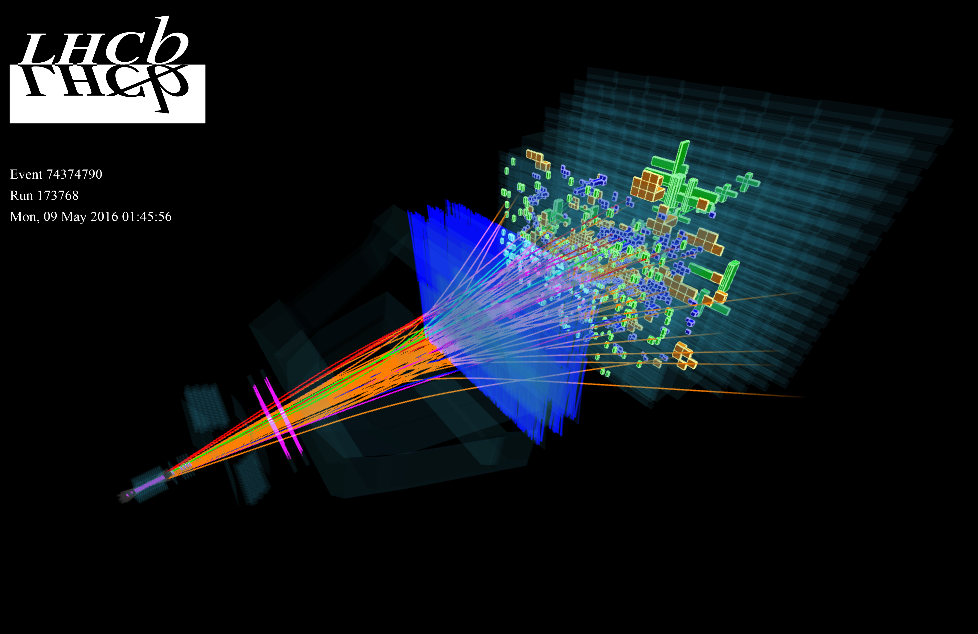
\includegraphics[scale=0.9]{figures/LHCb7_event.png}
\caption{A typical LHCb event fully reconstructed during data taking on May 9th 2016 (during Run II). Particles identified as pions, kaon, etc. are shown in different colours. Figure taken from \cite{LHCb_event_display}.
\label{fig:event display}}
\end{figure}


One of the analyses, which utilizes long-lived particles, is a study of time-dependent CP-violating asymmetries in $B_0 \rightarrow J/\psi K_S^0 $ decays. Measurement of time-dependent $CP$ asymmetries provides a valuable test of the Standard Model's flavor sector as well as an opportunity for discovery effects of physics beyond the Standard Model.  
 The study of this asymmetry in the $B_0 \rightarrow J/\psi K_S^0 $  decay mode provides a way to determine the effective $CP$ phase. The $CP$ violation asymmetry in $b \rightarrow c\bar{c}s$decays of the B mesons is caused by the interference between mixed and unmixed decay amplitudes.
 A state initially prepared as a $B^0$ can directly decay into $J/\psi K_S^0$ or can oscillate into a $\bar{B}$ and then decays into  $J/\psi K_S^0$. Taking the correction to the theoretical uncertainty, this amplitude is equal to twice the angle $\beta = arg [ -  \frac{V_{cd}V_{cb}^*}{V_{td}V_{tb}^*} ] $ of the Unitary Triangle. 


\begin{figure}[h]
\centering
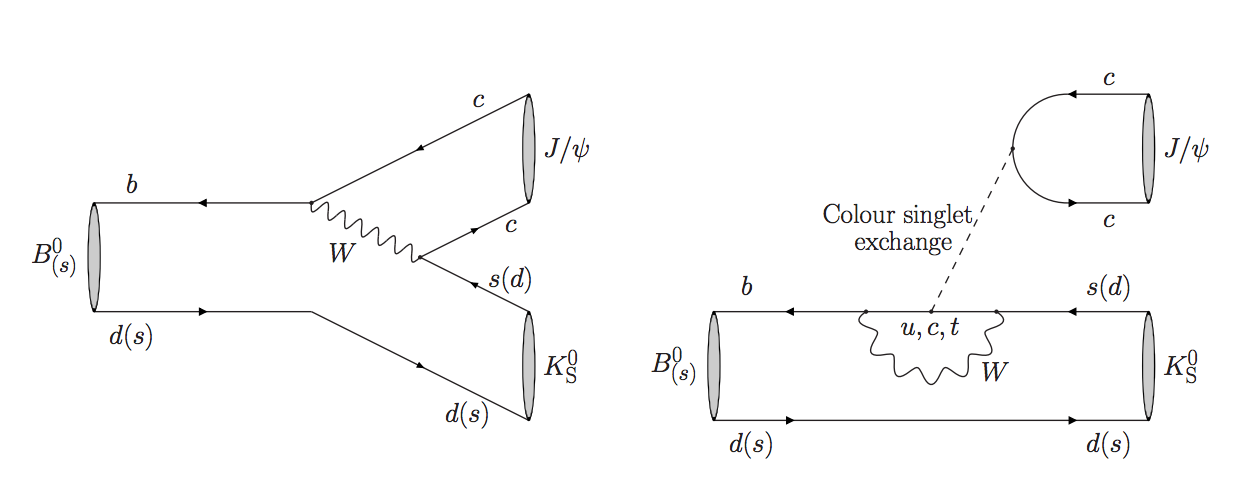
\includegraphics[scale=0.9]{figures/B0JPKs.png}
\caption{The Feynman diagram presenting the decay topologies contributing to the $B_0 \rightarrow J/\psi K_S^0 $ channel:  (left) tree diagram and (right) penguin diagram.
\label{fig:BJPSi}}
\end{figure}

\section{Downstream Tracking Algorithm overview}
\label{Sec:Downstrean Overview}
The description of the downstream tracking pattern recognition algorithm is based on \cite{patllt}. 

Downstream tracks at LHCb are reconstructed in the following way. First, a standalone track reconstruction in the T stations with an algorithm called PatSeeding is performed, creating T tracks, also called T-Seeds. 
Roughly speaking, the downstream tracking algorithm's goal is to add TT hits that are likely to match those T-seeds. 

After filtering with a machine learning classifier to discard bad candidates that are tracks that do not represent the trajectory of a real particle, these tracks are propagated back through the magnet to the TT station, described in great details in section \ref{sec:TT}, assuming they are coming from the point of origin of the coordinate system. 
Firstly, the pattern recognition algorithm searches for clusters in the two $x $-layers of the TT.  Those clusters already allow constraining the flight path of the particle with good precision. Then a cluster in the other $x$ layer is searched for. Finally, clusters in $U$ and $v$ layers are added. 
 Those selected clusters are then fitted to a parabola model using a $\chi^{2} $ minimization technique \footnote{Fitting a model to data involves the construction of a test statistic from the model and the data and minimizing that test statistics with respect to all parameters that are not considered fixed }. 
 The   $\chi^{2} $ is defined as :

\begin{equation}
\chi^{2}(\alpha) = \sum_{i=1}^{n} \frac{(f(x_i, \alpha)-x_i)^{2}}{\sigma_{i}^{2}}
\end{equation}
where  $\alpha$ us a vector of free parameters being fitted, $f(x_i;\alpha)$  is a model, and $\sigma_i$ are the uncertainties in the individual measurement $x_i$.  

To reduce spilover influence on a tracking reconstruction, a flag is set for each cluster if it is likely to have been created in a different collision than the current one.  This flag is called a high-threshold bit.  Tracks with a large number of high-threshold clusters are rejected. 
Finally, the best track is chosen according to the output of another multivariate classifier. 



\section{Downstream Track model}



\subsection{Propagation through the magnetic field}
\label{sec:magPoint}

Charged particles traversing through the tracking
stations, which are located outside of the magnetic field, follow a straight-line path. The bending of their trajectory inside the magnetic field can be approximated by a sharp kink in the flight path at a given $z$ position of a magnet point, called $z_{\text{mag}}$. The kink method is visualized in figure \ref{fig:magnetPointSketch}.
This $z$ position depends on the parameters of the track and is also affected by inhomogeneities in the field. The numerical value of this position can be obtained for the parametrized empirical formula: 
\begin{eqnarray}
\label{eq:zMag}
z_{\text{mag}} & = &\alpha_{0} + \alpha_{1} \cdot t_{y}^{2} + \alpha_{2} \cdot t_{x}^{2} + \alpha_{3} \cdot 1/p \\
& & +\, \alpha_{4} \cdot | x_{T} | + \alpha_{5} \cdot | y_{T} | + \alpha_{6} \cdot | t_{y} |. \nonumber
\end{eqnarray}
where , $t_{x}$ and $t_{y}$ are the slopes of the last track state in the
T stations. The absolute momentum, $p$, is
estimated from the T track, using a simplified parametrisation that assumes a kink of the trajectory at the center of the magnet and the track to come from the point of origin.
The observables $x_{T}$ and $y_{T}$ are the
$x$ and $y$ positions of the last state in the T stations, respectively. Analyzing equation \ref{eq:zMag}, one can find that the variable $z_{\text{mag}}$ depends mostly on the values in the first line, while the dependence on the ones from the second row is smaller.

\begin{figure}[!htbp]
 \begin{center}
    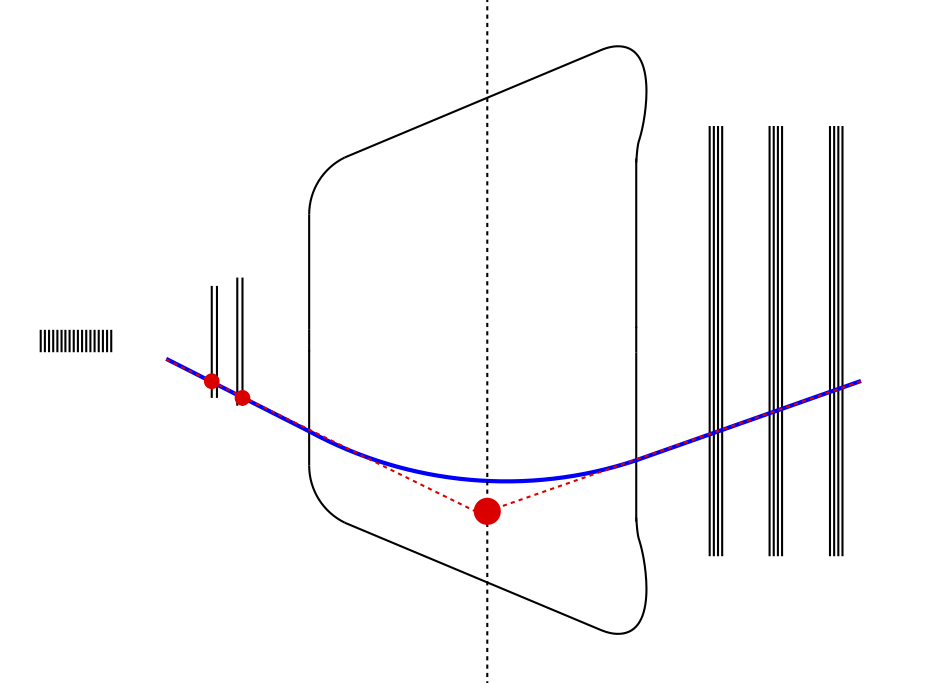
\includegraphics[width=0.49\linewidth]{figures/magnetPointDownstream2.png}
   \caption{Sketch of the LHCb detector with the tracking system in the $x$-$z$ plane. A downstream track (blue line) and its approximation outside the magnetic field (red dotted line) is shown. In the approximation the track undergoes a sharp kink at the magnet point (big red dot).
     \label{fig:magnetPointSketch}}
 \end{center}
\end{figure}


The $\alpha$ parameters are determined in using Monte Carlo simulations. Those numbers are obtained by fitting a straight line to the true position of the hits in TT, and a third-order polynomial to the true
position of the hits in the T stations. The crossing point of both curves in the $x$-$z$ projection
determines the \textbf{true} value of $z_{\text{mag}}$. An illustration of $z_{\text{mag}}$ determined in described way, and
the difference between the values obtained with equation \ref{eq:zMag} when using measured 
instead of simulated quantities are shown in figure \ref{fig:zMag}.

\begin{figure}
 \begin{center}
   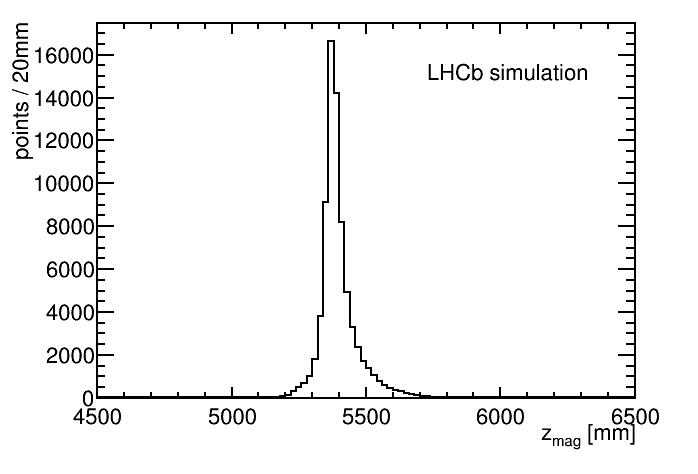
\includegraphics[width=0.49\linewidth]{figures/zMag.png}
    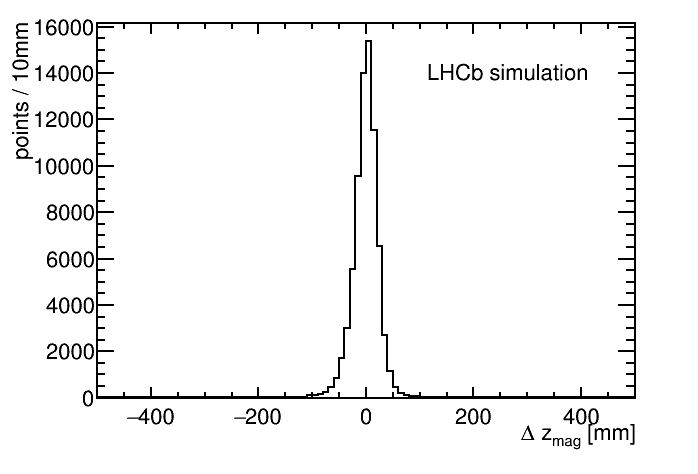
\includegraphics[width=0.49\linewidth]{figures/deltaZMag.png}
   \caption{Left: <<True>> z position of the magnet point. Right: Difference
   between true and estimated $z$ position of the magnet point. For the true position, simulated observables, for the estimated position measured observables were used.
     \label{fig:zMag}}
 \end{center}
\end{figure}

The $x$ position of the magnet point is then determined by using a linear extrapoltion of the
state in the T stations to $z_{\text{mag}}$.
\begin{equation}
x_{\text{mag}} = x_{T} + t_{x} \cdot (z_{\text{mag}} - z_{T})
\end{equation}

 
To correct the effect of magnetic filed on estimation of the $y$ position, an additional correction is applied:

\begin{equation}
\label{eq:ymag}
y_{\text{mag}} = y_{T} + t_{y} \cdot (z_{\text{mag}} - z_{T}) - \beta_{1} \cdot t_{y} \cdot \Delta_{\text{slope}}^{2}
\end{equation}
where $\Delta_{\text{slope}}$ is the difference of the slopes in $x$ before and after the magnet, defined as: 
\begin{equation}
\Delta_{\text{slope}} = \left| x_{\text{mag}}/z_{\text{mag}} - t_{x} \right|,
\end{equation}
and $\beta_{1}$ an empirical parameter.

The predicted slope in $y$ in the TT is calculated as:

\begin{equation}
t_{y,TT} = t_{y} \cdot (1 + \beta_{0} |t_{y}| \Delta_{\text{slope}}^{2})
\end{equation}
with  $\beta_{0}$ an empirical parameter, determined on simulation, 
using regression with true observables, to correct
for the effect of the bending in the magnetic field on the slope in $y$.


The track that constitutes of OT hits only requires a dedicated procedure since $y$ resolution, and the resolution of the slope in $y$ is rather poor. 
Thus, the following parametrization is used instead:
\begin{eqnarray}
y_{TT} & = & y_{T} + t_{y} \cdot (z_{\text{mag}} - z_{T}) + t_{y,TT} \cdot (z_{TT} - z_{\text{mag}}) - \beta_{1} \cdot t_{y} \cdot \Delta_{\text{slope}}^{2},
\end{eqnarray}
where $\beta_{1}$ is determined on simulated data using regression with true observables. 
The current implementation of the algorithm does not apply any further track correction logic, therefore the slope in the T stations can be calculated as:
\begin{equation}
t_{y, \text{constr}} = y_{T} / ( z_{T} + (\beta_{0} |t_{y}| z_{\text{mag}} + \beta_{1} ) \Delta_{\text{slope}}^{2})
\end{equation}

For tracks with hits in the OT only, corrected $t_{y, \text{constr}}$ is used in equation \ref{eq:ymag} instead of the measured value $t_{y}$.

Determination of the magnet point is crucial since it is used as an additional constraint in the downstream track $\chi^{2}$ fit, see section \ref{sec:chi2}. Therefore, its uncertainty has to be determined and those are calculated by estimating the difference between the values of $x_{\text{mag}}$ and
$y_{\text{mag}}$ obtained using simulated quantities and reconstructed quantities for the extrapolation. This uncertainty depends on $\Delta_{\text{slope}}$ and the types of hits that constitute the track. 
The following empirical parametrisations of the uncertainty
were used:
\begin{eqnarray}
\sigma_{x, OT} & = & (2.0 + 18.0\cdot \Delta_{\text{slope}})\mm \nonumber \\
\sigma_{y, OT} & = & (5.0 + 20.0\cdot \Delta_{\text{slope}} + 50\cdot \Delta_{\text{slope}}^{2})\mm  \nonumber \\
\sigma_{x, IT} & = & (1.0 + 16.0\cdot \Delta_{\text{slope}})\mm  \nonumber \\
\sigma_{y, IT} & = & (2.0 + 15\cdot \Delta_{\text{slope}})\mm  \nonumber
\end{eqnarray}
The numerical values of those parameters were obtained by fitting residual distributions.

\subsection{Determination of the momentum}
The momentum of a downstream track mainly depends on the kink it undergoes in
the magnetic field, but also shows a dependence on the slopes in $x$ and $y$.
The following parameterisation results in a momentum resolution of about 2\%
averaged over the momentum spectrum.
\begin{eqnarray}
\label{eq:momentum}
p & = & \frac{ \gamma_{0} + \gamma_{1} \cdot t_{x}^{2} + \gamma_{2} \cdot t_{y}^{2} }{ \Delta_{\text{slope}} },
\end{eqnarray}
where again the parameters $\gamma_{i}$ were determined using the true position
of the hits in simulation. This resolution contains both the effect from the detector 
resolution and from dependencies which are not accounted for in the parametrization. 
The momentum resolution is presented in figure ~\ref{fig:momReso}.
\begin{figure}[!htbp]
 \begin{center}
   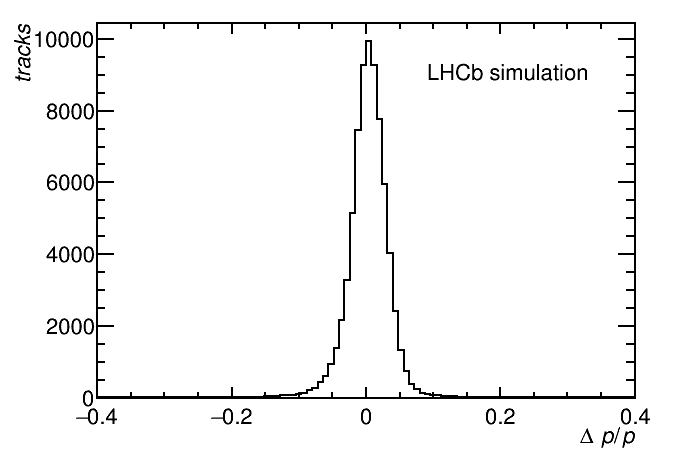
\includegraphics[width=0.8\linewidth]{figures/momReso.png}
    \caption{Momentum resolution for the initial track estimate. It amounts to about 2\%.
     \label{fig:momReso}}
 \end{center}
\end{figure}


\subsection{Track model in the TT}
\label{sec:trackModelTT}
The downstream track is modeled as a parabola in the TT. This representation comes from the presence of a strong residual magnetic field in and before the TT, which deflects low-momentum particles from a straight-line trajectory. 
The track is modeled by the following function:

\begin{equation}
\label{eq:track_in_tt}
x(z) = x_{0} + t_{x} \cdot (z - z_{\text{mag}}) +c \cdot (z - z_{TT})^{2},
\end{equation}
with $z_{TT}$ the $z$ position in the middle of the TT, $z_{mag}$ the $z$
position of the magnet point, $t_{x} $ the slope in $x$ in TT, and
$c= 1.48\cdot 10^{-5} \cdot \Delta_{\text{slope}}$. The initial value for $x_{0}$ is $x_{\text{mag}}$.
 
The parameter $c$ is determined on simulation by fitting the true position of the hits in TT with a parabola and determining it as a function of $\Delta_{\text{slope}}$. The deflection from a straight line is tiny. For instance, a track with a momentum of $3 GeV/c^{2}$, is deflected of about $200\mu m$, which is roughly the strip pitch of a TT sensor.

The $y$ position of the track is modeled as a straight line: 
\begin{equation}
y(z) = y_{0} + t_{y,TT} \cdot (z - z_{\text{mag}}),
\end{equation}
where $t_{y,TT} $ is the track's slope in $y$ given by equation \ref{eq:track_in_tt}, and  the initial value for $y_{0}$ is $y_{\text{mag}}$. 

\section{Pattern Recognition}

This section provide an overview of the stages of the pattern recognition in LingLivedTracking, which are presented in the figure \ref{fig:PatLL}. The detailed description on the first step, filtering T seeds, was moved into the separate section  \ref{sec:TSeed}. 

\begin{figure}
\centering
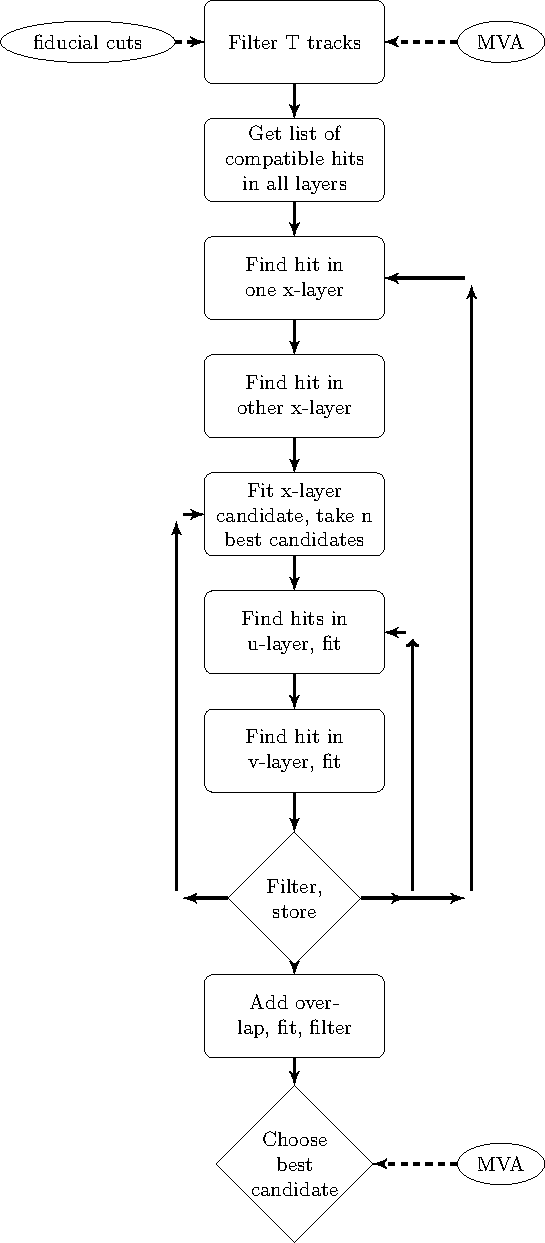
\includegraphics[scale=0.7]{figures/PatLL.pdf}
\caption{Different stages of pattern recognition within the  PatLongLivedTracking algorithm. 
\label{fig:PatLL}}
\end{figure}


\subsection{T-seeds reconstruction}
The algorithm, that performs pattern recognition for the T-seeds is called PatSeeding \cite{PatSeeding}. It consists of five distinct steps: 

\begin{itemize}
\item hit preparation;
\item track search per detector region;
\item track search for tracks migrating from IT to OT;
\item track search per Outer Tracker region for tracks at large $|y|$;
\item validation of low-quality tracks left over from the per region search;
\end{itemize}

Within this algorithm, the track is described as a straight line in $x-y$ plane.  For $x-z$ projection, a cubic model with three parameters is used:
\begin{eqnarray}
x(z)&=&c(z-z_{reference})^2(1+d_{ratio}(z-z_{reference})) + b(z-z_{reference})+a \\
y(z)&=&b_{y}z+a_y
\end{eqnarray}

$d_{ratio}$ describes the correlation between the quadratic and cubic terms and is determined from
Monte Carlo studies. The shift by $z_{reference}$ makes the fit more numerically stable ($z_{reference}$ is
in the middle of the T stations, by default).

\subsection{Search for compatible hits}
In this initial reconstruction stage, the downstream track candidates are modeled by the straight line from the LHCb origin point (0,0,0) to the magnet point, which is the only constrain. 
This model is not always accurate since most particles of interest do not originate from the global LHCb origin (0,0,0), thus a correction to the $x$ position of the search window is applied.  The value of the search window is given by: 
\begin{equation}
\delta x = \text{sign}(p\cdot \text{magPol}) \cdot \left( \texttt{XCorrectionConst} / p + \texttt{XCorrectionOffset} \right),
\end{equation}
with magPol the magnet polarity. This correction is  shown in figure ~\ref{fig:preselWindow}, left. 
 
Furthermore, a similar search window technique was applied to momentum-dependent search, which can be seen in figure  \ref{fig:preselWindow}. The
dependence of the window size on the momentum is given by:

\begin{equation}
\Delta x = \texttt{XPredTolConst} / p + \texttt{XPredTolOffset},
\end{equation}
where $p$ is the absolute value of the momentum. The parameters determining the
size of the search window, \texttt{XPredTolConst} and
\texttt{XPredTolOffset}, were derived on simulation, illustrated on the right of
figure \ref{fig:preselWindow}.

\begin{figure}[!htbp]
 \begin{center}
  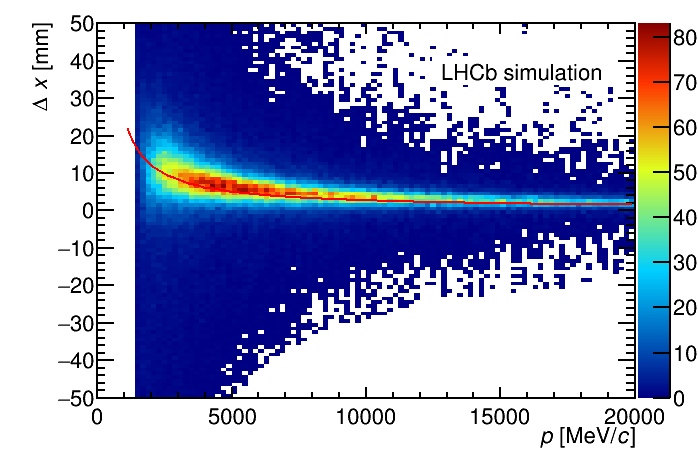
\includegraphics[width=0.49\linewidth]{figures/xPosCorrection1.png}
   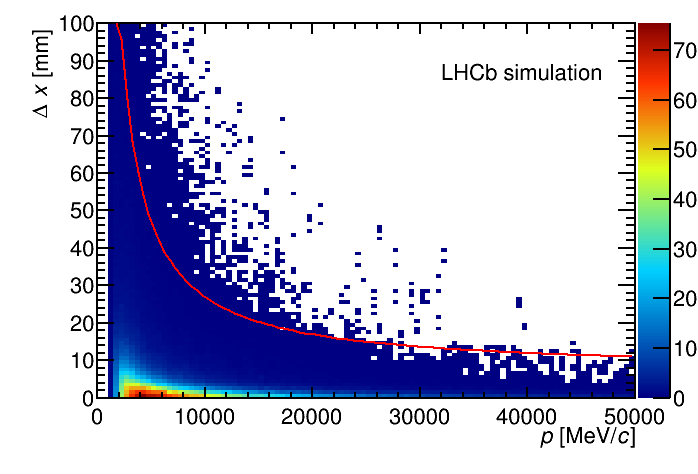
\includegraphics[width=0.49\linewidth]{figures/preselWindow1.png}
   \caption{Left: Distance between extrapolated track (constrained to come from the LHCb origin (0,0,0)) and (truth-matched) hits
   before correction. The red line represents the correction function which is
   applied. Right: Distance between extrapolated track and (truth-matched) hits
   as a function of the momentum of the track for the preselection step, after
   the correction. The cut is show as the red line.
     \label{fig:preselWindow}}
 \end{center}
\end{figure}


Finally, the pattern reconstruction algorithm checks whether the hit is compatible with the expected $y$-position in the TT with a tolerance \texttt{YTol}. As the position of a hit in the TT can only be determined up to
the length of a sensor module, this provides only a weak constraint. The $x$
positions of the hits in the stereo layers are then updated, assuming the $y$ position from the T track extrapolation.

All hits in all four layers which lie inside these tolerances are then stored in a container, and
sorted according to the projection distance, this is the absolute distance of the hit to the predicted position.

The T track is not considered if less than three hits in the TT are found in
total, or the $x$ or the stereo layers do not contain any hit.


\subsection[Search for hits in $x$ layers]{Search for hits in {\boldmath $x$} layers}
In this step, the algorithm iterates over all hits preselected by the previous step hits in the $x$ layers to form preliminary track candidates.  

The first hit that is added to the track candidate is chosen in one of the two $x$ layers. This allows for a more precise
determination of the slope of the track and the curvature, and therefore also of the momentum of
the partially reconstructed downstream track.

 Next, corresponding hits in the other $x$ layer are
searched for. The search window in the other $x$ layer is defined as follows:

\begin{equation}
\Delta x =  \texttt{TolMatchConst} / p + \texttt{TolMatchOffset} ,
\end{equation}
if $\Delta x$ is smaller than a given value \texttt{MaxWindowSize}, otherwise
\texttt{MaxWindowSize} is taken as the tolerance. This serves as a sanity check
to exclude unphysically large values of the window size for low momentum
particles. All hits within this window are then considered for further
processing. As illustrated in the left hand plot of figure ~\ref{fig:matchingDist}, 
essentially all hits from true particles
in simulation are enclosed within this region.

\begin{figure}[!htbp]
 \begin{center}
  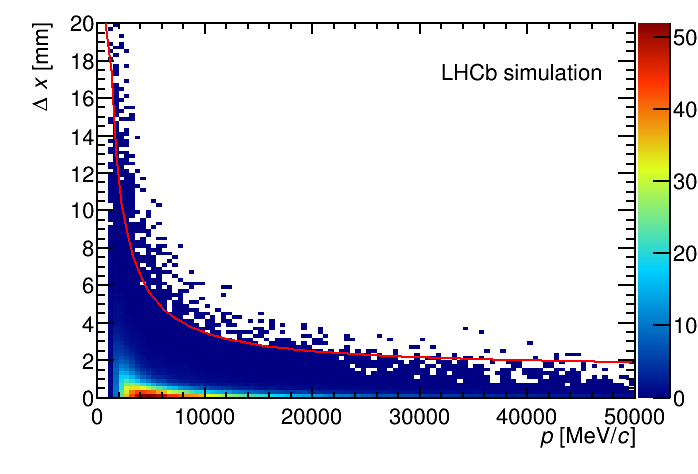
\includegraphics[width=0.49\linewidth]{figures/matchingDist1.png}
  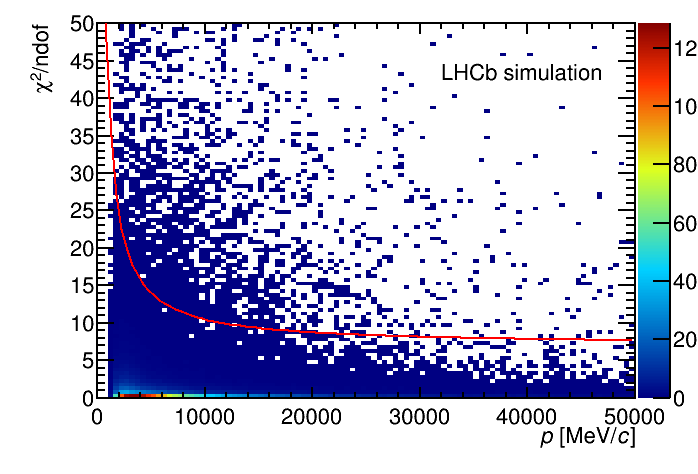
\includegraphics[width=0.49\linewidth]{figures/xChi2Cut1.png}
   \caption{Left: Distance between extrapolated track with one $x$ hit and
   (truth-matched) hit in the other $x$ layer. The red line represents the cut
   on the distance. Right: $\chi^{2}$ values for a fit to the $x$ hits
   (truth-matched), with the cut represented as a red line.
     \label{fig:matchingDist}}
 \end{center}
\end{figure}


A $\chi^{2}/ndf$ fit to the $x$ coordinate is then performed for each possible candidate, consisting
of the first hit in the $x$ layer, and one of the matching hits in the other $x$
layer. The magnet point is used as a further point to add enough degrees of freedom for the fit. All track candidates are then sorted according to their
$\chi^{2}/ndf$  value, and track candidates are discarded if the $\chi^{2}/ndf$  value is
above:

\begin{equation}
\chi^{2}/\text{ndf}_{\text{max, x hits}} =  \texttt{FitXProjChi2Const} / p + \texttt{FitXProjChi2Offset}.
\end{equation}
If no hit could be found in the other $x$ layer, the track candidate is not rejected. 
It is kept without fit to search for hits in the $u$ layer. This allows for hit inefficiencies in the TT.

Due to the large combinatorial background, there can be many ghosts in this selection.
Track candidates with only two $x$ hits are prone to be ghost tracks, and it is possible that the true combination of hits does not have the smallest $\chi^{2}/ndf$ .
Therefore, in the next steps, the first \texttt{MaxXTracks} candidate has considered whose $\chi^{2}/ndf$  value is within the range
(\texttt{MaxChi2DistXTracks}) to the lowest $\chi^{2}/ndf$  value.

In future studies, this section can be enhanced by training a machine learning model to select the best matching hits. 

\subsection[Search for hits in the $u$ layer]{Search for hits in the {\boldmath$u$} layer}

The search window in the $u$ layer can be smaller than 
those in the $x$ layers, since the parameters of a track with two hits are reasonably well constrained. 
 Hits are searched around the track extrapolated to the
$u$ layer, where the $x$ position of the hit is updated by using the
extrapolated $y$ position. All hits within a search window are
considered, where the window size is defined as

\begin{equation}
\label{eq:uTol}
\Delta x =  \texttt{TolUConst} / p + \texttt{TolUOffset}.
\end{equation}
The parameters \texttt{TolUConst} and \texttt{TolUOffset} are determined
from simulation, visualized in the left hand plot of figure \ref{fig:uvLayerDist}.
The hits inside the window are then sorted according to their distance between the extrapolation of the track and their actual position. For each hit which passes this tolerance, a new track candidate is formed, until the maximum number of $xu$
tracks (\texttt{MaxXUTracks}) is reached. Each of these candidate is then fitted
with a $\chi^{2}$ fit to obtain the best parameters for the final search in the $v$ layer.


\subsection[Search for hits in the $v$ layer]{Search for hits in the {\boldmath$v$} layer}
The last step in the hit search subroutine is searching for the hits in the $v$.  If the track's candidate already has three hits, a momentum dependent window is created according to the following formula: 

\begin{equation}
\Delta x =  \texttt{TolVConst} / p + \texttt{TolVOffset}.
\end{equation}
Figure \ref{fig:uvLayerDist} (right) ilustrate this this search window. In case the track only contains two hits,
formula \ref{eq:uTol} is used to determine the size of the search window.
The hit that is closest to the extrapolation is added.


\begin{figure}[!htbp]
 \begin{center}
  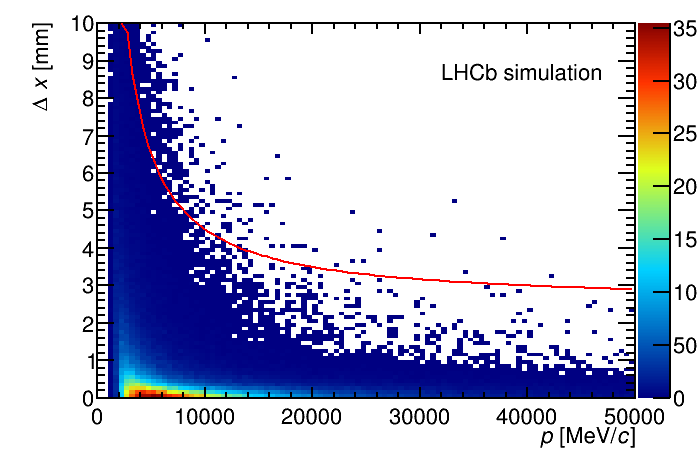
\includegraphics[width=0.49\linewidth]{figures/deltaXULayerCut1.png}
  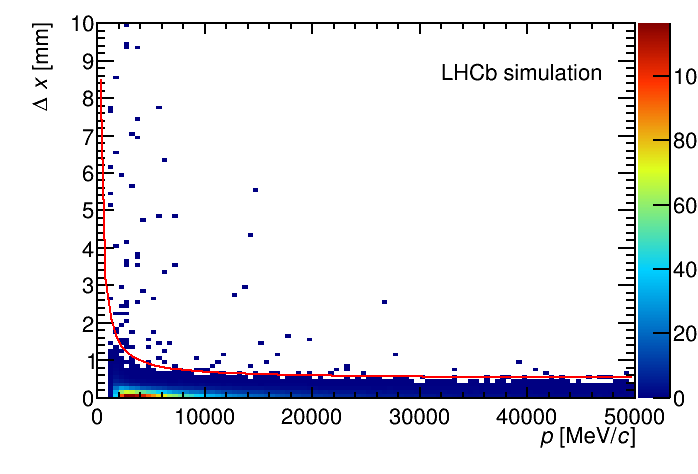
\includegraphics[width=0.49\linewidth]{figures/deltaXVLayerCut1.png}
   \caption{Left: Distance between extrapolated $x$-hits track and
   (truth-matched) hit in $u$ layer. The red line represents the cut on the
   distance. Right: Distance between extrapolated $xu$-hits track and
   (truth-matched) hit in $v$ layer. The red line represents the cut on the distance.
     \label{fig:uvLayerDist}}
 \end{center}
\end{figure}



\subsection[Calculation of $\chi^{2}$ and outlier removal]{Calculation of {\boldmath$\chi^{2}$} and outlier removal}
\label{sec:chi2}
At this stage, all possible hits in TT were added to the track candidates. It is the time to perform a $\chi^{2}$ fit. If the fit $\chi^{2}/ndf$ is smaller than a given value (\texttt{MaxChi2} and \texttt{MaxChi2ThreeHits} for candidates with four and three hits, respectively, 
the candidate is accepted and passed on to the next stage. Otherwise, the hit that contributes most to the $\chi^{2}$ is removed, and the fit is repeated. 
The procedure is repeated until either the $\chi^{2}/ndf$  is small enough, 
or alternatively, there are hits in less than three planes left.
Furthermore, for each iteration of the fit, an explicit sanity check is made
that each hit is still compatible with the estimated $y$ position of the track.
The $\chi^{2}$ is defined as:

\begin{equation}
\chi^{2} = \sum_{i \in hits} \frac{ \left(x_{i} - (x_{0} + t_{x}\cdot(z-z_{mag}) + c \cdot (z - z_{TT})(z - z_{TT}) + \left( \frac{dx}{dy} \right)_{i} y_{0}) \right)^{2}  }{\sigma_{i}^{2}}
\end{equation}
with $\left( \frac{dx}{dy} \right)_{i}$ the slope of the stereo plane and
$y_{0}$ the displacement in $y$. Note that $c$ is fixed, see section \ref{sec:trackModelTT}.

\begin{figure}[!htbp]
 \begin{center}
  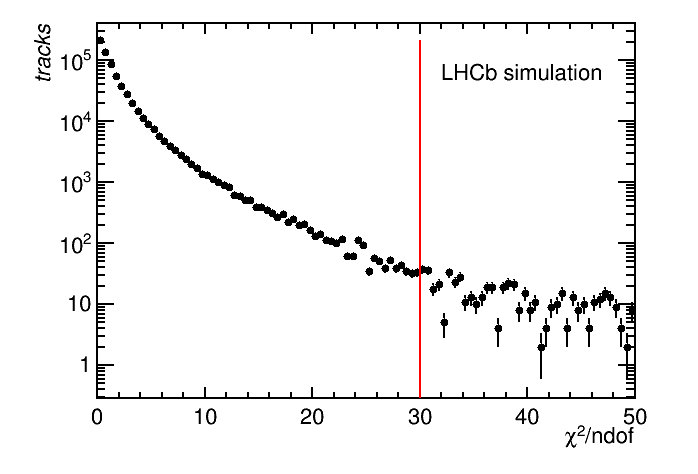
\includegraphics[width=0.49\linewidth]{figures/chi2Cut1.png}
  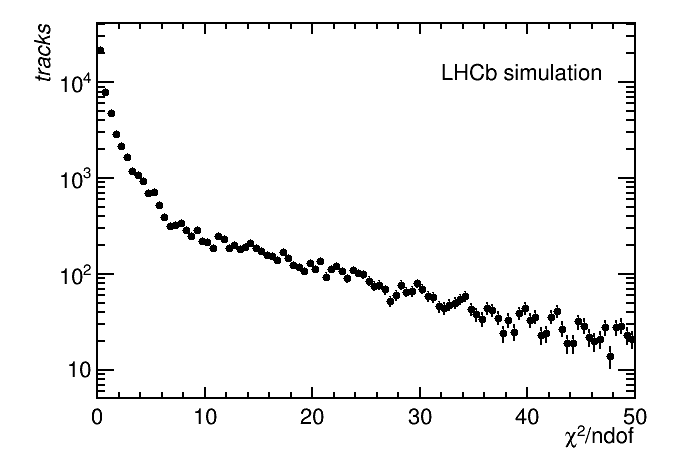
\includegraphics[width=0.49\linewidth]{figures/chi2Cut3Hits1.png}
   \caption{Left: $\chi^{2}$ distribution for truth-matched tracks with 4 or more
   hits. The maximum allowed value is 30. Right: $\chi^{2}$ distribution for
   truth-matched tracks with 3 hits. The maximum allowed value is 50.
   \label{fig:chi2Cuts}}
 \end{center}
\end{figure}





\subsection{Accepting the candidates}
\label{sec:acceptCandidate}
The track candidate is accepted in the final selection of track candidates,
if it fulfills the following criteria. All cut values were obtained using simulated data, 
with the goal of keeping a balance between signal retention and background rejection. 

\begin{itemize}
\item It has at least three hits in at least three different layers of the TT.
\item The $\chi^{2}/ndf$is below a given threshold. This value is different for
three-hit tracks (\texttt{MaxChi2ThreeHits}) and tracks with four or more hits (\texttt{MaxChi2}),
see figure \ref{fig:chi2Cuts}. 
\item It contains at least as many hits as any other candidate for a given T track.
\item The track has a pseudorapidity larger than 1.8 and smaller than 5.2.
\item At least \texttt{NMinHighThresHits} of the hits have the high-threshold
bitset.
\end{itemize}

The following checks are repeated, this time using the fit result instead of the initial estimates.

\begin{itemize}
\item The momentum estimate is compatible with the momentum estimate from the
T track.
\item The track has a minimum momentum \texttt{MinMomentum} and a minimum $p_{T}$ \texttt{MinPt}.
\item The track does not point into the beampipe.
\end{itemize}

\subsection{Addition of overlap hits}
\label{sec:addOverlap}
For all track candidates whose are retained at this stage, hits in the overlap
regions of the TT detector are searched for. 
TT modules are staggered in the $z$ direction with an overlap, in order to cover the insensitive region of the modules and not to lose efficiency. A hit qualifies as an overlap hit if it
is within a certain distance to the extrapolated track (\texttt{OverlapTol}), in the same
layer as an already existing hit, but at a
different $z$ position.

As adding an extra hit will change the track's properties, the track
is again fitted with the potential removal of outliers. 


\section{Selection of T tracks }
\label{sec:TSeed}

T-seeds together with TT hits constitute an input to the LongLivedTrackign (LLT) algorithm and their quality has a direct and significant impact on the algorithm performance. Therefore, the very first and crucial step is a filtering procedure, which purpose is to increase purity of the set of T-tracks by rejecting as many unreconstructible track as possible. This also allows to reduce the execution time since the combinatoric is greatly reduced. A previous analysis showed that T-seed filtering based on a simple linear selection using track quality and kinematic variables is not feasible. Therefore, an idea of using Machine Learning techniques was proposed. This section is dedicated to present all studies, starting from preparing and understanding training dataset, to selecting the best model, to attempting to understand the model's prediction. 

This problem is similar to the email spam detector, in both cases it is desired to keep all true events and remove as much as possible false events. The nature of this problem reflects in selection of the cutoff probability threshold.  

\subsection{T-seed classifier: Data Collection} 

The very first step within the training Machine Learning model pipeline is a data collection. It is not possible to build any statistical model without collecting sufficient amount of data. From the perspective of this project the data was generated by the Monte Carlo simulation. To extract required data a dedicated tool within Brunel project was implemented. This tool is dedicated to match track with MC particle. The particle is considered as matched to a given track if they share at least 70\% of the hits. Such a link allows to assign a target value to tracks.    

One of the most difficult problem during the data preparation step was choosing the track labeling policy. Within this process, for each T-seed a target flag was assigned. What is crucial, every time when a strategy is changed, the entire process of model selection and training has to be redone, which happens at least three times during author's study. The final labelling strategy tells the track is consider as a reconstructable, later called a \textbf{true T-seed}, when it meets the following criteria:
\begin{itemize}
    \item Has to be associated with a valid Monte Carlo particle;
    \item From above association the electron is excluded; 
    \item Has at least two hit associated with TT station;
    \item no hits in the Velo detector. 
\end{itemize}

Those criteria can be justified by definition of the Downstream tracks, which are created by the particles that decays outside of the Velo detector. 

\section{T-seed classifier Exploratory Data Analysis}

The next step that were performed is Exploratory Data Analysis. This step is essential to understand the input data, find patterns, relationships, or anomalies that can influence the outcome of the model prediction.   

\begin{figure}
\centering
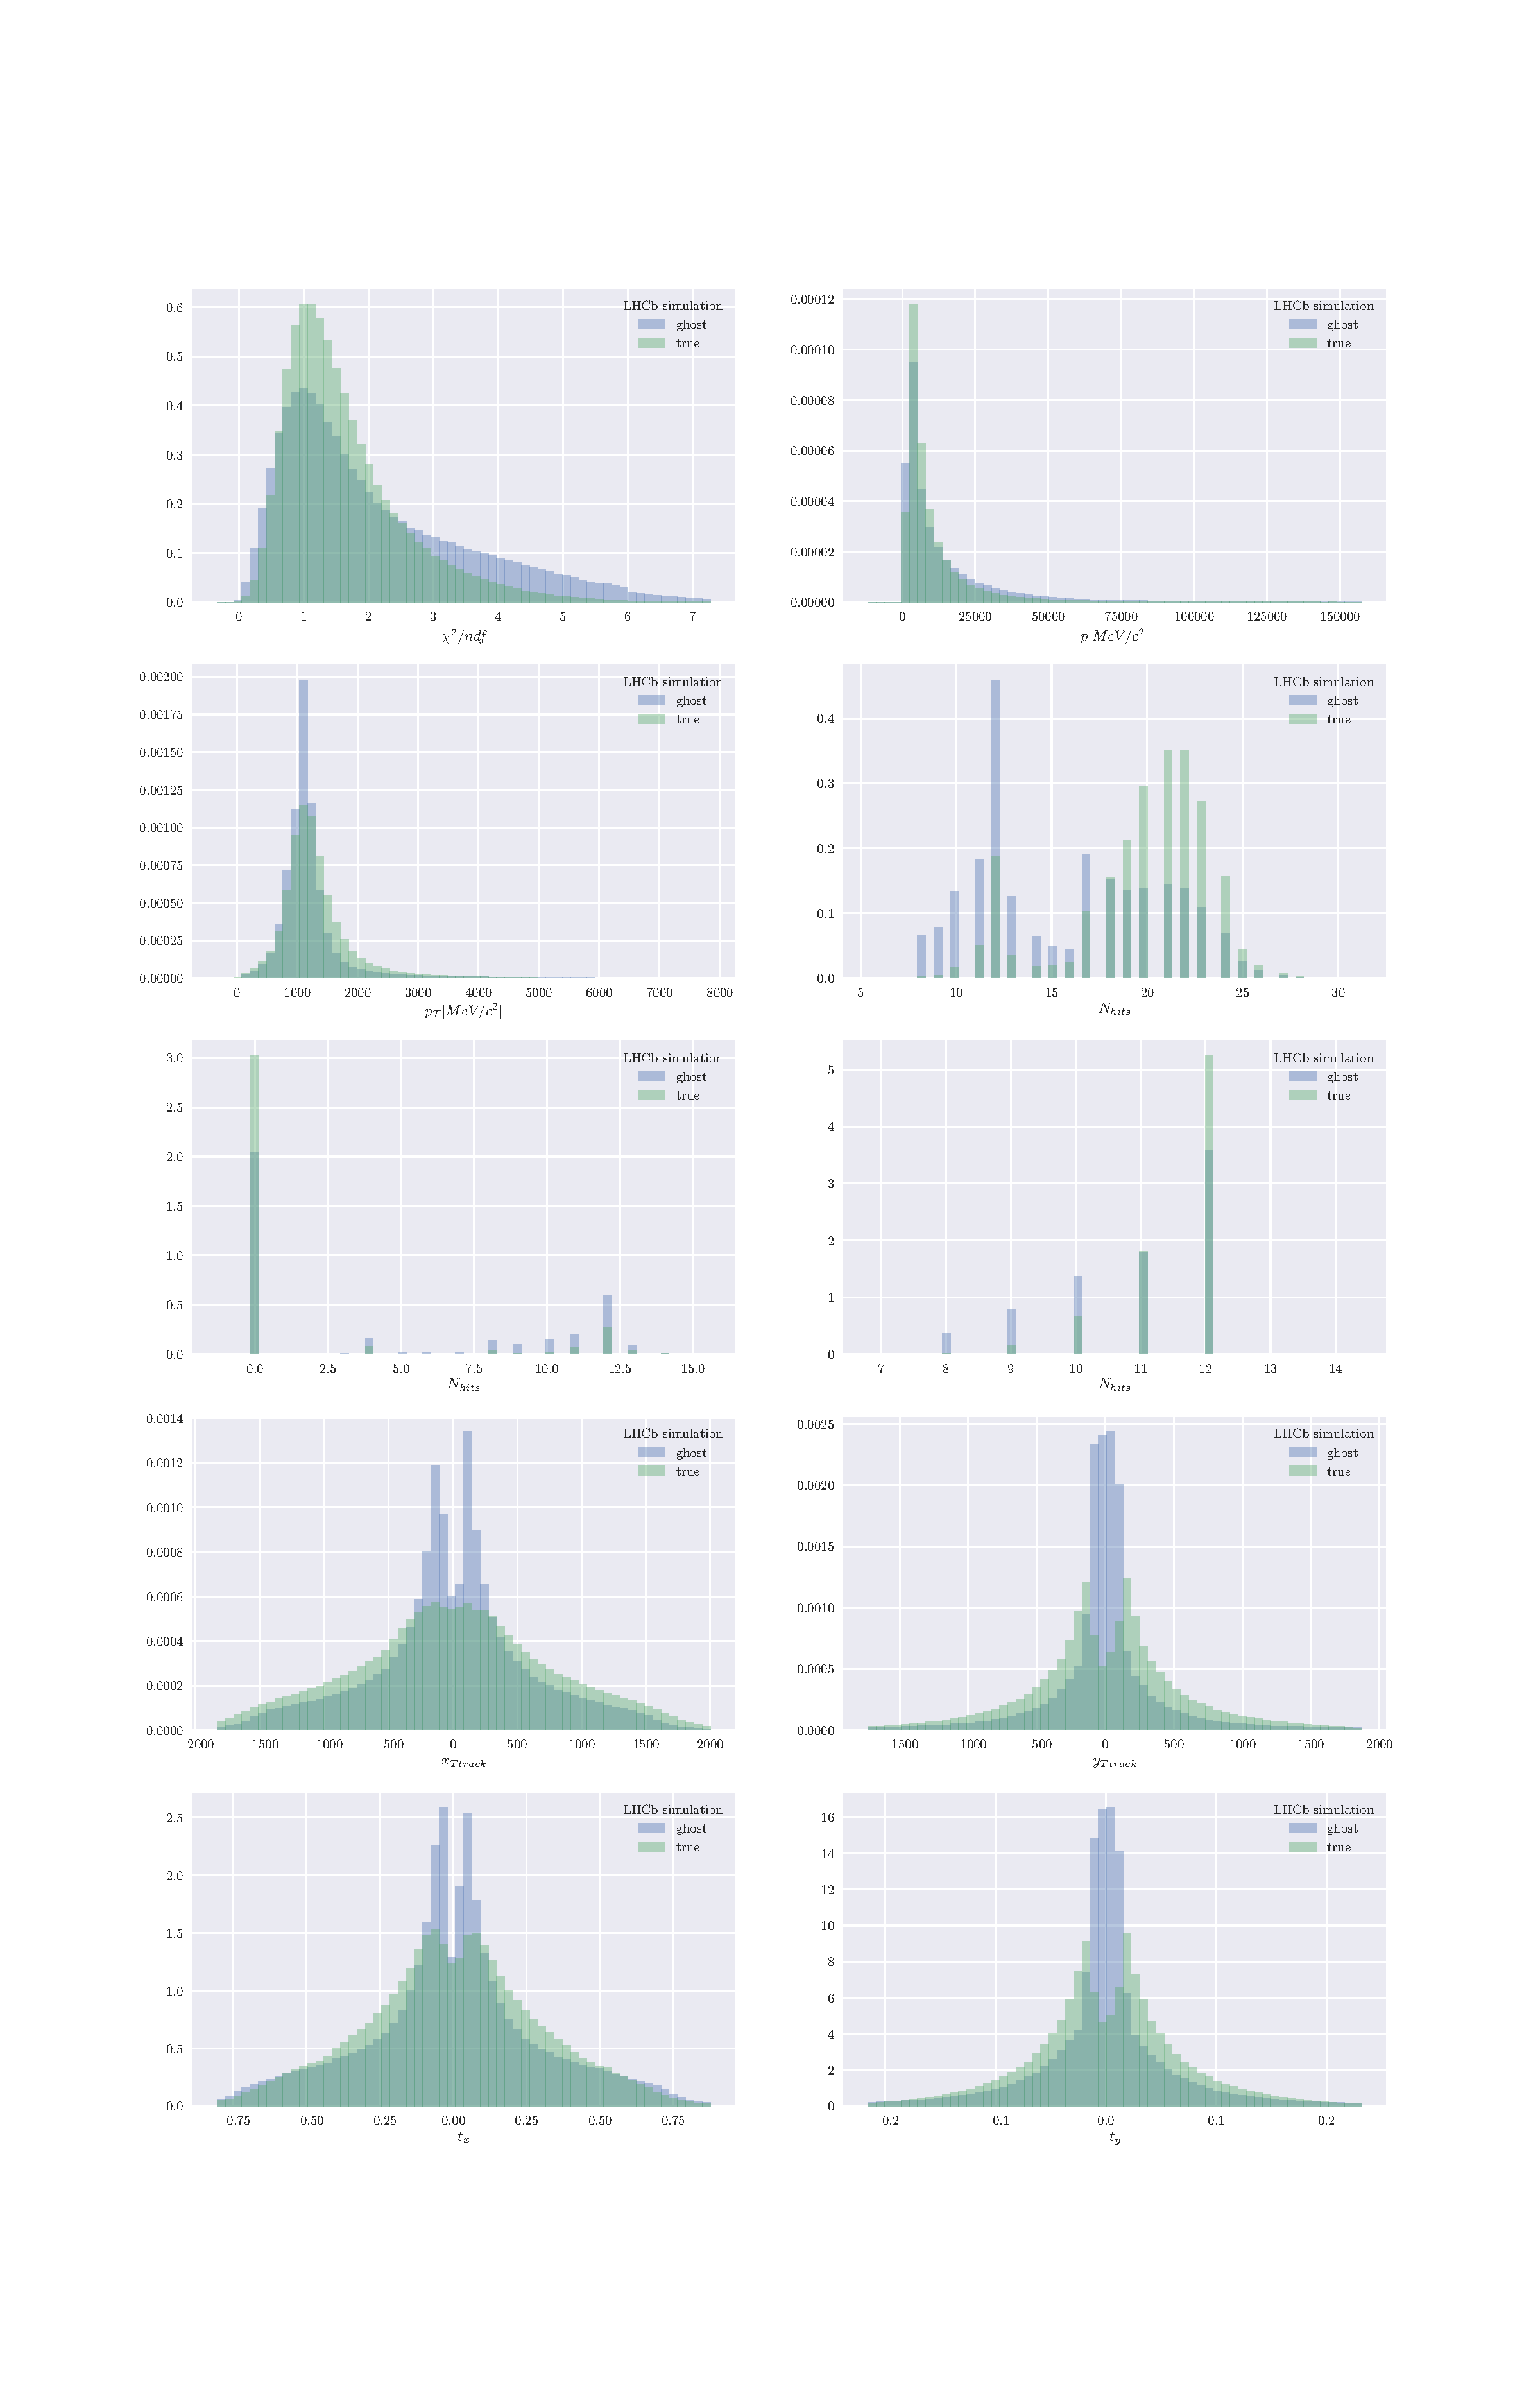
\includegraphics{figures/features.pdf}
\caption{Distribution of the input variables used to train T-Seed filter. The sample was extracted using a $B_0\rightarrow J/\psi K_S^0 $ samples decays. The green solid histogram is the signal distribution, while the light blue
distribution is the background.
\label{fig:input features}}
\end{figure}

The search for the best classifier was performed using a simulated data sample containing signal events $B^0\rightarrow J/\psi K_S^0 $ decays events. The entire dataset contains more than 2 million T-Seeds. TO avoid bias that could be introduced by considering only one magnet polarization the training dataset contains the data of both magnet polarities.  
The following variables were considered as an initial features set. Further input dimentionality enhancement was done in the feature engineering phase. 

\begin{itemize}
    \item $\chi^2/ndf$: T-track $\chi^2/ndf$ determined by the PatSeeding algorithm, which is defined in the following way: 
    \begin{equation}
        \chi^2 = \sum_{hits i} \frac{1}{\sigma_i^2} \left( \frac{x_i-x_{track}(z_i)}{\cos \alpha} \pm r_{drift} \right) 
    \end{equation}
    where: $(x_i, z_i)$ is the $x$ coordinates of the i-th hit at the $y(z_i)$ predicted form the track model, $\sigma_i$ is the hit postilion uncertainty and $r_{drift}$ is the drift radius for Outer Tracker hits or 0 for the Inner Tracker. 
    \item $p$: the absolute momentum of a T-track; 
    \item $p_t$: the transverse momentum;
    \item $N_{hits}$: number of hits constructing tho a given T-seed;
    \item $x_{T track}$: the $x$ position of the T track's first state; 
    \item $y_{T track}$: the $y$ position of the T track's first state;
    \item $t_x$: the slope of the track in the $x-z$ plane;
    \item $t_y$: the slope of the track in the $y-z$ plane;
    \item $r_{track}$: the distance from the beam line, z-axis, calculated for the first state. The $r_{track}$ is calculated as follow:
    \begin{equation}
        r_{track} = \sqrt{x_{T track}^2 + y_{T track}^2}
    \end{equation}
    \item $\eta$: pseudorapidity. 
\end{itemize}
Each of above feature distributions is presented in the figure \ref{fig:input features}. It is clearly visible that the data is not linearly separable and the distribution for both true and false classes are very similar to each other. 

One of the most popular way to show the dependencies among features is to calculate  the Pearson correlation coefficient $\rho$. The formula for $\rho$ is:

\begin{equation}
    \rho(X,Y) = \frac{\mathbb{E}(X-\mu_x)(Y-\mu_y)}{\sigma_x \sigma_y}
\end{equation}

This parameter has value in the range of $<-1,1>$. The value of 0 indicates no correlation, the -1 and 1 implies strong negative and positive correlation respectively. In order to visualize all of the correlation coefficients, so called correlation matrix was created. Figure \ref{fig:corrMatrix} shows two correlation matrices, the data separation was done according to the target flag. There is no significant difference between true and false T-Seeds correlation matrices. This gives the first impression, that the classification task is hard. 

\begin{figure}
  \centering
  \begin{tabular}{@{}c@{}}
    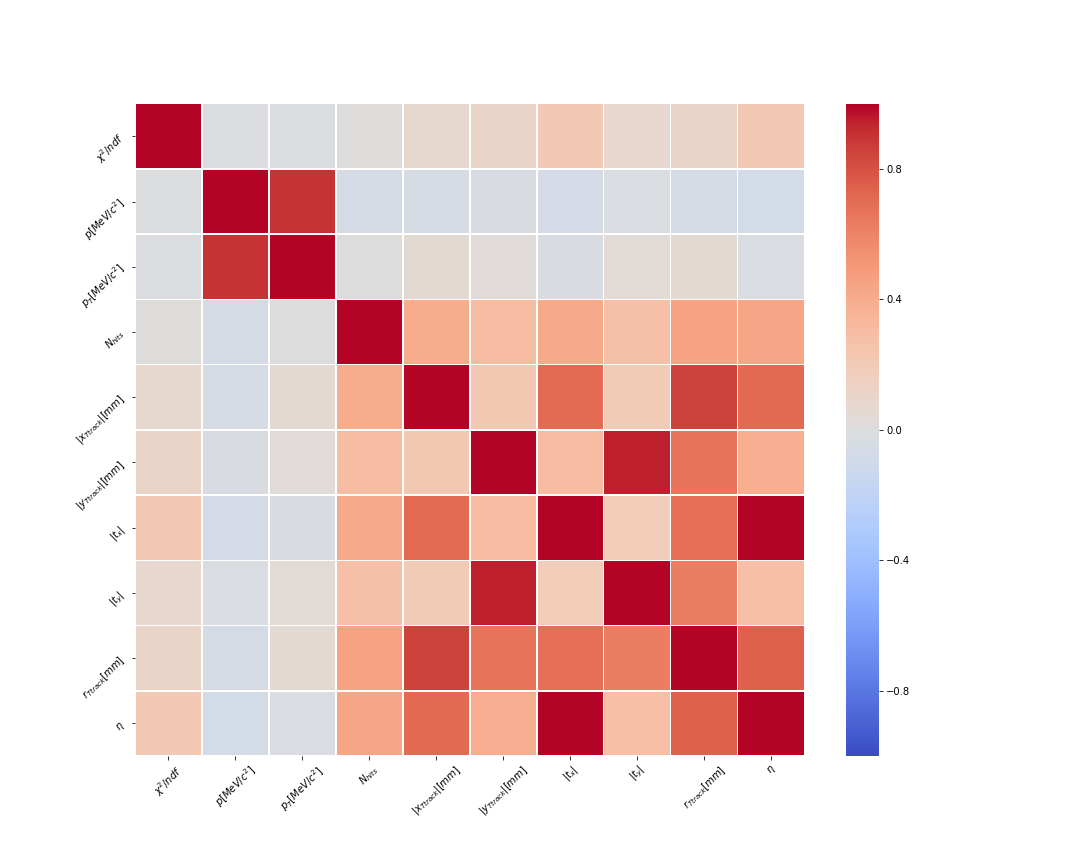
\includegraphics[width=\linewidth]{figures/corr_matrixTrue.png}
  \end{tabular}

  \vspace{\floatsep}

  \begin{tabular}{@{}c@{}}
    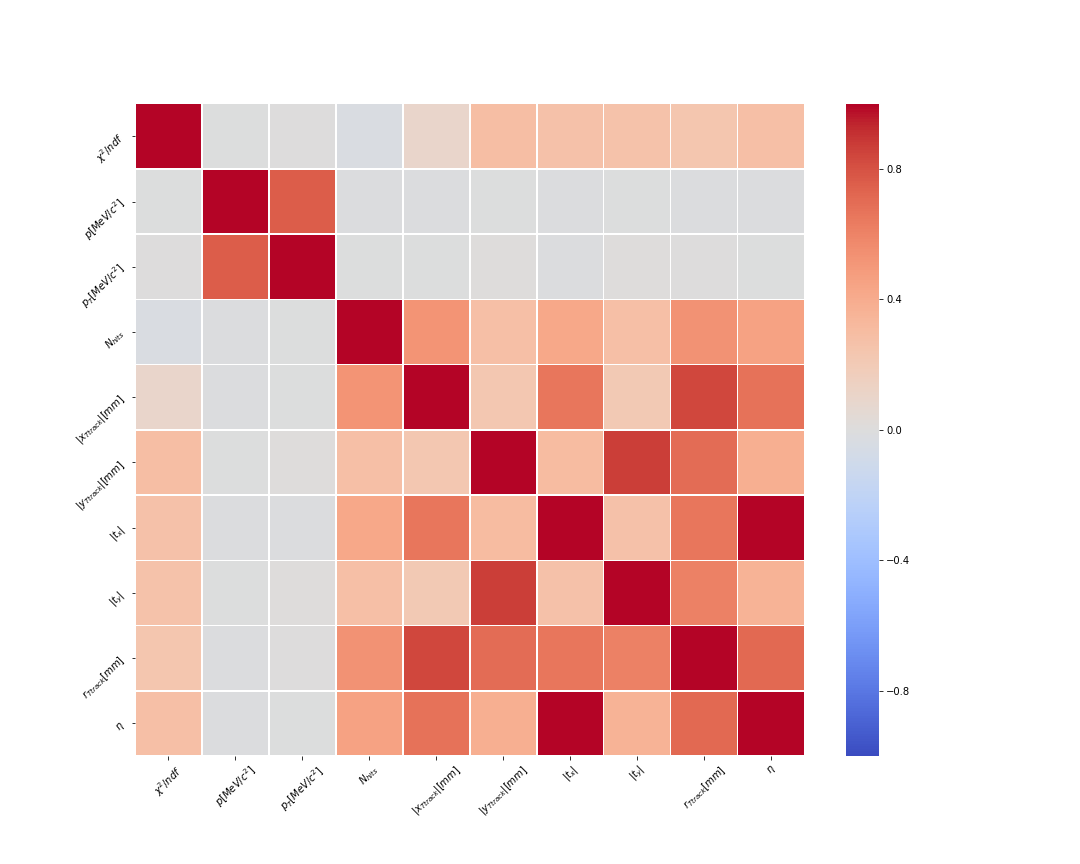
\includegraphics[width=\linewidth]{figures/corr_matrixFalse.png}
  \end{tabular}

  \caption{Pearson  correlation matrix that were obtained using a subset of input features. The top plot shows correlation matrix for True T-seeds. The bottom plot presents similar Pearson correlation matrix generated using the ghost T-Seeds.  
\label{fig:corrMatrix}}  
\end{figure}

    
The Pearson  correlation coefficient is a good metric to detect linear dependencies among features, but it is not sensitive to more sophisticated relations. To overcome this limitation the pair-plot was made, showed in figure \ref{fig:Pair plot}. A pairs plot allows to see both distribution of single variables and relationships between two variables, which is carried as a scatter plot. This is particularly interesting to visually inspect how the variables are distributed for a given pair of attributes. To make this plot more readable the data were split into two groups according to the target flag. That kind of plot allows to make an initial guess on the features importance. 

\begin{figure}[!h]
\centering
\hspace*{-2cm}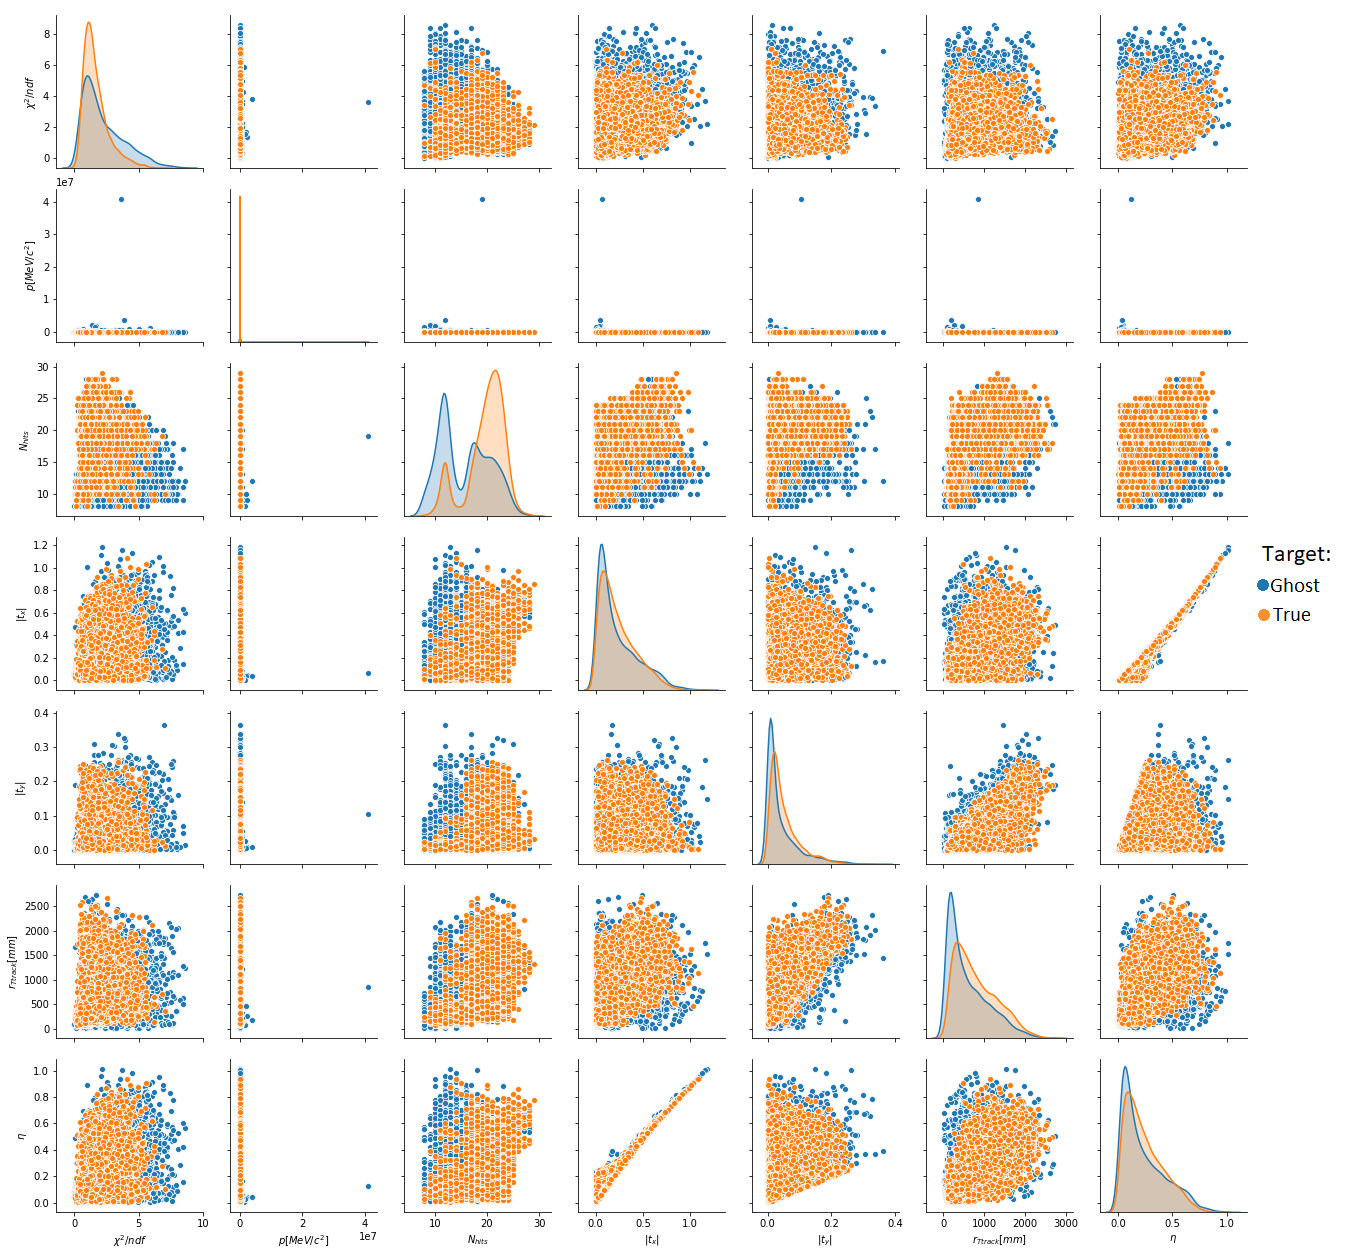
\includegraphics[width=1.3\textwidth]{figures/pair_plot.png}
\caption{Pair-plots that were generated using subset of input features. The input data was separated based on the value of the target flag. The blue points represents ghost T-Seeds and the orange points represents true T-Seeds. }
\label{fig:Pair plot}
\end{figure}

\section{T-Seed classifier: baseline}

This section dedicated to present the Machine learning study baseline, which was implemented as training of two models, kNN and logistic regression.
 
These two models were selected as a baseline due to their simplicity and a short amount of time that is required to train them. The simplicity, except for the model's underlying idea, is manifested by a small number of hyperparameters that needs to be tuned. The baseline score is the entry point to the Machine Learning study. This score  should be over-performed by all of the more sophisticated models. It also provides an initial understanding of how hard the classification problem is. In some cases, excluding this one, the baseline could be an average human performance on the task. 

\subsection{$k$NN} 
\label{sec:KNN_result}

The $k$NN described in section \ref{sec:knn}, is a model that has two hyperparameters that need to be selected - a number of neighbors and the distance metric. The training pipeline contains of the following steps:

\begin{itemize}
    \item Data extraction;
    \item Data normalization: each of the features were normalized by removing the mean and scaled to unit variance. Centering and scaling happen independently on each feature by computing the relevant statistics on the samples in the training set. 
\end{itemize}
The mentioned pipeline were implemented using sklearn framework\cite{sklearn}.  

Figure \ref{fig:kNN score} presents the ROC AUC score versus the number of neighbors. The score and its uncertainty were obtained using the cross-validation method. The classifier's score maximum value, ROC auc score 76, were obtained for $k \approx 210$.  

\begin{figure}[!h]
\centering
\hspace*{-1cm}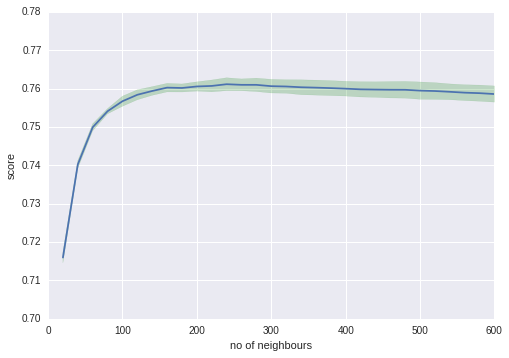
\includegraphics{figures/knn.png}
\caption{The kNN performance plot, ROC auc score vs the number of neighbor. The green shaded area represents score's one standard deviation region.}
\label{fig:kNN score}
\end{figure}

\subsection{Logistic Regression}

The second baseline mode is Logistic Regression described in section \ref{sec:LogReg}, and implemented using sklearn framework.
The input to this model has to be normalized, which is the only preprocessing step that was applied, therefore the data processing pipeline was identical to the one described in section \ref{sec:KNN_result}. 
To maximize the classifier score analysis of the L1 and L2 regularization constants were conducted. These two hyperparameters were introduced to reduce overfitting, although as presented in figure \ref{fig:RL_L1} none of them has significant impact on the classifier performance.


\begin{figure}[h]
  \centering
\begin{tabular}{c c}
\subfloat{{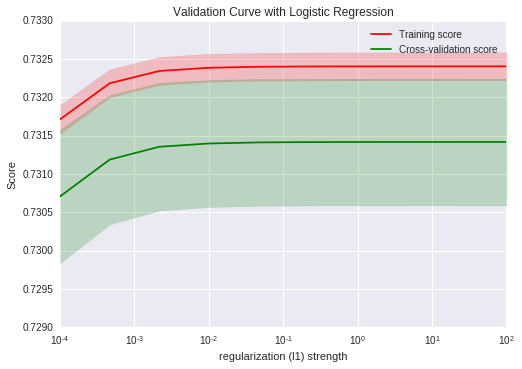
\includegraphics[width=0.5\textwidth]{figures/RL_L1.png} }}%
    \subfloat{{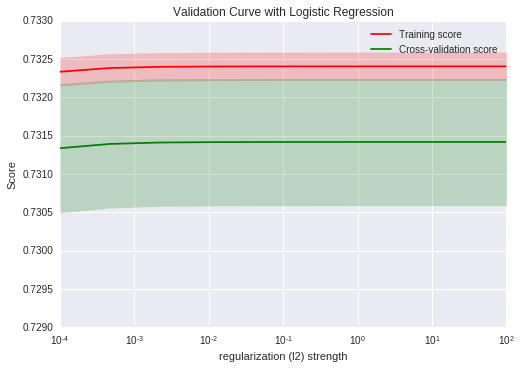
\includegraphics[width=0.55\textwidth]{figures/RL_L2.png} }}%
\\
\end{tabular}
   \caption{Logistic Regression validation curves. The plots present the impact of L1 (left) and L2 (right) regularization on classifier performance.  
\label{fig:RL_L1}}  
\end{figure}

  
Finally, to check the stability of the prediction, the study of model performance versus a number of training entries was performed. The results are shown in figure \ref{fig:LR_NE}. This plot indicates the biggest limitation of the linear model. The model’s performance is not affected by increasing the amount of data, that were used to train them.  

\begin{figure}[!h]
\centering
\hspace*{-1cm}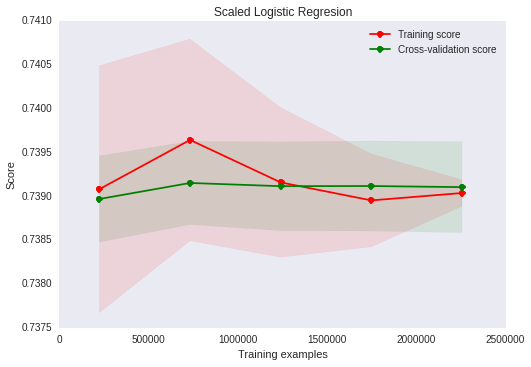
\includegraphics{figures/LogReg_te.png}
\caption{The Logistic Regression model performance vs. the number of training examples}
\label{fig:LR_NE}
\end{figure}

The score, measure as ROC AUC, obtained by the Linear Regression model is about 74\%, which is slightly worst than the result obtained by the kNN classifier.  

\section{T-Seed classifier: study based on XGBoost model}

The previous two models were selected to provide the baseline scores. This section presents the training strategy and results that were obtained using the XGBoost model. 

The first step within this analysis was to train the model with default values of hyper-parameters to get a better understanding of the model initial performance. This step was also executed to estimate the number, or at least the order of magnitude, of weak learners that need to be added to the boosting model. This number can be estimate by detecting moment when model performance starts to saturate. 

The model saturation is a situation when adding a new tree has no positive impact on the performance, measured on both training and the validation datasets. This effect can be easily detected using a learning curve plot. The learning curve plot is a two-dimensional plot with classifier performance on the y-axis and a number of trees on the x-axis. The saturation effect occurs when learning curve Plateau. 

The initial training allows estimates of the number of trees to be around 700. The other hyperparameters, that were taken into consideration are listed below:

\begin{itemize}
    \item \textbf{learning rate} - shrinkage parameters (see section \ref{sec:xgboost}), which control the weight of new tree added to the model;    
    \item \textbf{max depth} - a maximum allowed depth of each of the trees, increasing its value makes week learners more complex and more likely to overfit. 
    \item \textbf{gamma} - minimum loss reduction required to make a further partition on a leaf node of the tree. Increasing the gamma values makes the boosting process more conservative. 
    \item \textbf{min child weight} - a minimum sum of instance weight needed in a child to make a split. If the tree partition procedure step produces a leaf node with a sum of instance weight smaller than \textbf{min child weight}, then the building tree process is terminated. This parameter can be interpreted as a minimum number of instances needed to be in each node.
    \item \textbf{colsample by tree} - subsample ratio of features used to construct a particular tree. Subsampling occurs once for each tree. 
    \item \textbf{reg alpha, reg lambda} - regularization factor L1 and L2 on weights.      
    
\end{itemize}

Taking into consideration the dimensionality of this optimization problem, as well as the fact that each training iteration takes about 1 hour the Bayesian Optimization seemed to be the most promising approach to tune the hyperparameters. Although, all three hyperparameters tuning strategies described in section \ref{sec:hyperparameters} were applied. Figure \ref{fig:hyperparameter_xgboost} presents the Bayesian optimization results in a form of coverage plot, where each of the scores is a ROC AUC score calculate using three-fold cross-validation method. Within the presented experiment the Gaussian process was selected as a surrogate function and Expected Improvement played the role of an acquisition function. Each training round was terminated once the performance on the test dataset has not improved after a fixed number of training iterations. This method is called early stopping, and its main purpose is to prevent training the model when it performance saturates. The positive site effect of this method is reduction of overfitting. 

The Bayesian optimization needs about 40 iterations to find the optimal hyperparameter set \footnote{In this context \textbf{optimal} is consider to be the best one for a given subset of hyperparameter's ranges, it is not guaranteed to be globally optimal}. The Grid and Random Search provide similar results, although each of these methods requires more optimization steps to find a set that works as good as the one produced by Gaussian optimization. 

\begin{figure}
\centering
\hspace*{-1cm}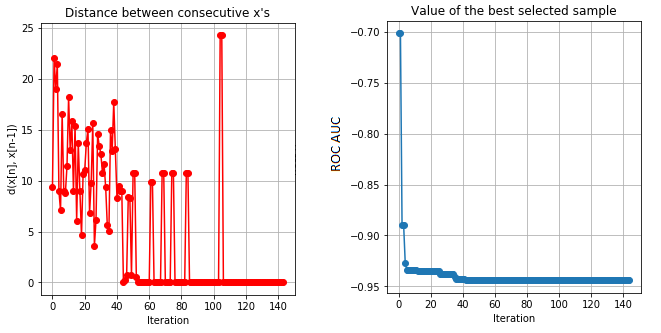
\includegraphics{figures/GaussianOptXgboost.png}
\caption{Bayesian optimization coverage plots. The left plot presents iterations vs. distance between consecutive selected hyperparameters sets, the right plot shows iterations vs. the ROC auc score of the current model.}
\label{fig:hyperparameter_xgboost}
\end{figure}

Using selected by the Bayesian optimization method set of hyperparameters, the final xgboost based model achieved a score, measured as an area under the ROC curve of 94\%. The figure \ref{fig:xgboost trainig} presents three different learning curve plots. The first one shows the training progress measured as a reduction of the cross-entropy loss versus the number of trees constituted the model. The second one presents the binary classification error rate, which is calculated as a ratio between a number of wrongly classified cases to all test cases, vs the number of training iterations. The final one presents how the area under the ROC curve versus number of weak learners. The learning curve plots were obtained using a test sample that constitutes 20\% of the entire dataset. 


\begin{figure}
\centering
\hspace*{-1cm}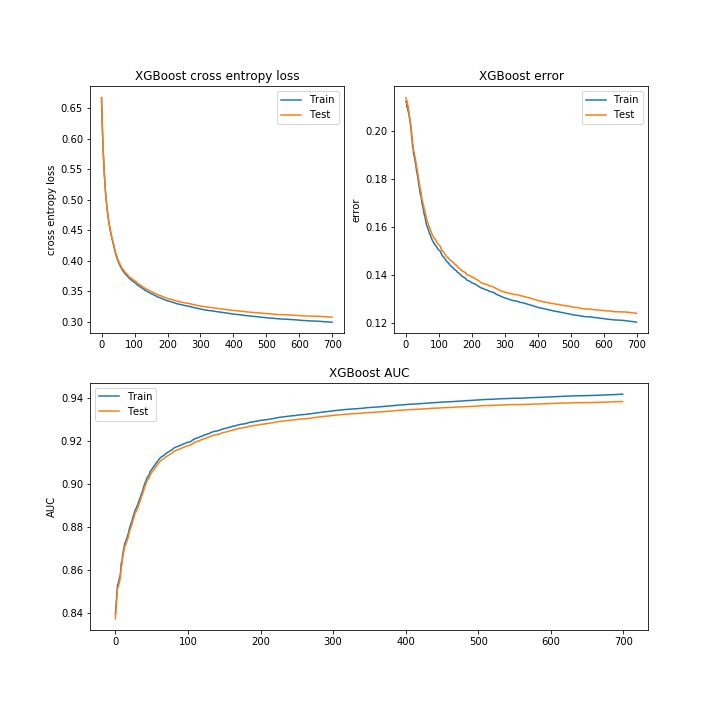
\includegraphics{figures/learning_curve_xgboost.png}
\caption{Learning curve for the XGBoost classifier. The upper left plot presents cross-entropy loss function vs. a number of week estimators, the right upper plot shows miss classification vs the number of trees. The bottom plot presents how the ROC AUC versus training iterations.}
\label{fig:xgboost trainig}
\end{figure}


The learning curve plot is one of the most important tool to visually investigate whether model is overfitted.  
Overfitting refers to a model that has learned the training dataset too well, including the statistical noise or random fluctuations in the training dataset. This effect becomes apparent when the performance gap between training and validation curves increase when increasing the model complexity, which is shown in figure \ref{fig:xgboost_overfitting} .Figure \ref{fig:xgboost trainig} clearly indicates that the model perform very well and the effect of overtraining is not present \footnote{This conclusion is based on a specific testset, that constitutes examples comming from the same distribution.}. 


\begin{figure}
\centering
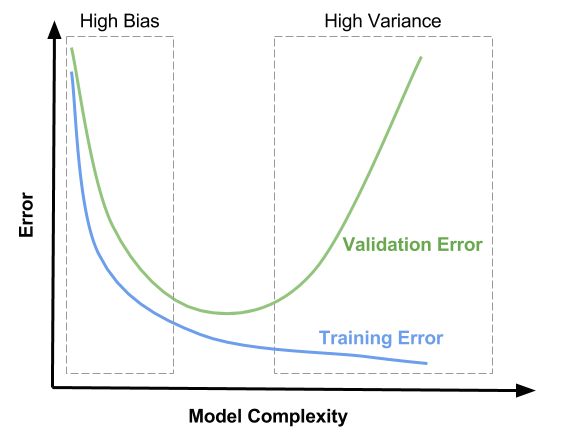
\includegraphics[scale=0.6]{figures/bbdt_overfitting.png}
\caption{Cartoon presenting different behaviour of the Boosted Decision Tree classifier. The leftmost region represents the model that is undertrained which is reflected in decreasing learning curves. The rightmost region corresponds to the model that is overtrained, in such a case validation curve is increasing while train curve is decreasing. }
\label{fig:xgboost_overfitting}
\end{figure}



\section{T-Seed classifier as a bonsai Boosted Decision Tree }

As described in section \ref{sec:bbdt}, the evaluation of the continuous complex classifier is too expensive (from the perspective of CPU time) to deploy that kind of model within HLT2. Therefore, the model was binarized and deployed in the form of bBDT, which is visualized in figure \ref{fig:bbt_structure}. 



\begin{figure}[h]
\centering
\hspace*{-1cm}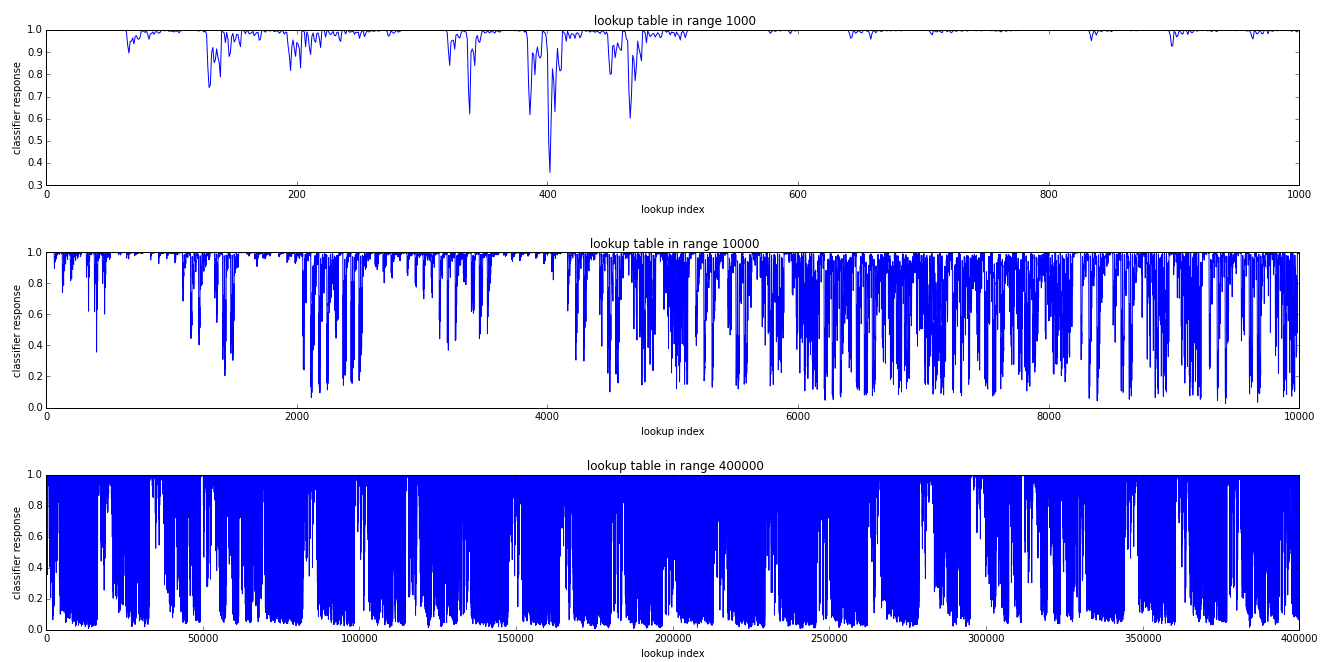
\includegraphics{figures/BBDT_lookup.png}
\caption{Structure of the bBDT lookup table. Each of the plot presents different range of lookup tables (x-axies) versus reposnse of the classiers (y-axies).}
\label{fig:bbt_structure}
\end{figure}



The response of the binned BDT and its ROC curve are presented in figures  \ref{bbdt response} and \ref{fig:ROC binned} respectively. A slight drop in the performance of the binned classifier with respect to the full one has been noted. The figures of merit measured for the bBDT algorithm amounted to 87\%. Based on the ROC curve the classification threshold was selected to be $0.07$, see section \ref{sec:CUT finetuning} for more details. This highly conservative value of the threshold was advocated by the fact that the final classifier has to keep more than 99\% of the true seeds. Nevertheless, this threshold value allowed to remove 30 \% of the fake seeds, thus significantly decrease the ghost rate, formally defined in section \ref{sec:physic_performance}.   



\begin{figure}
\centering
\hspace*{-1cm}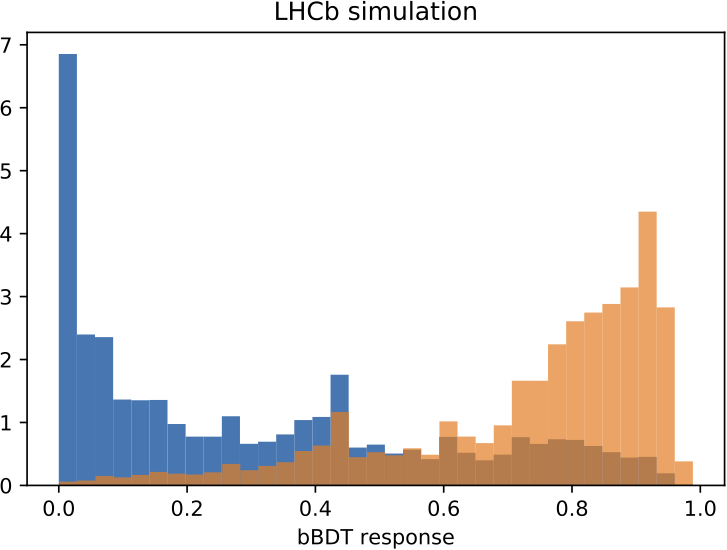
\includegraphics[scale=0.6]{figures/bbdt_response.png}
\caption{bBDT classifier output distribution, blue is background and orange is signal }
\label{fig:bbdt response}
\end{figure}


\begin{figure}
\centering
\hspace*{-1cm}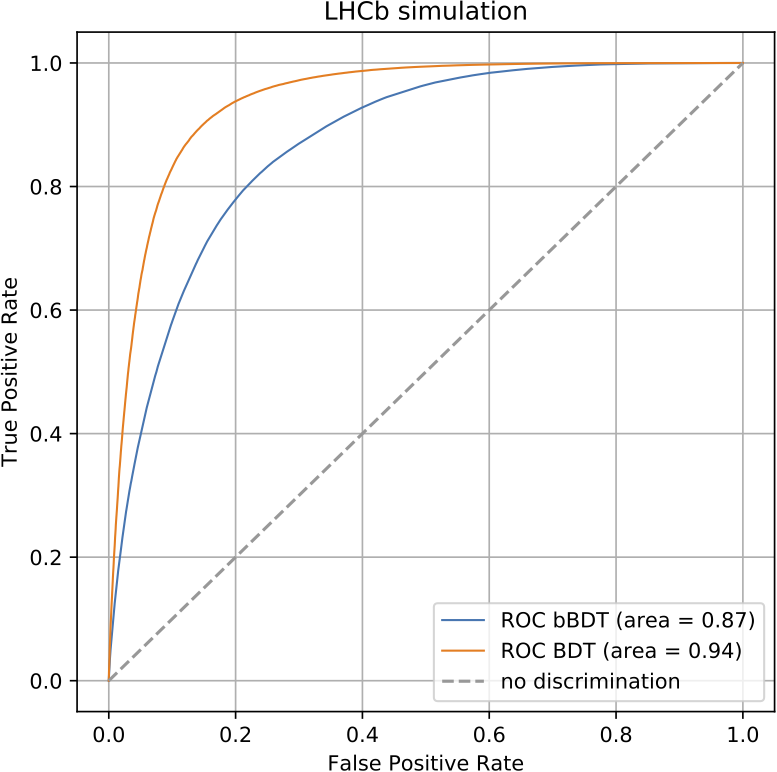
\includegraphics[scale=0.6]{figures/bBDT_roc.png}
\caption{Comparison of ROC curves for selecting true T tracks using a simulated $B_0\rightarrow J/\psi K_S^0 $ sample before and after binning.}
\label{fig:ROC binned}
\end{figure}


\begin{figure}
\centering
\hspace*{-1cm}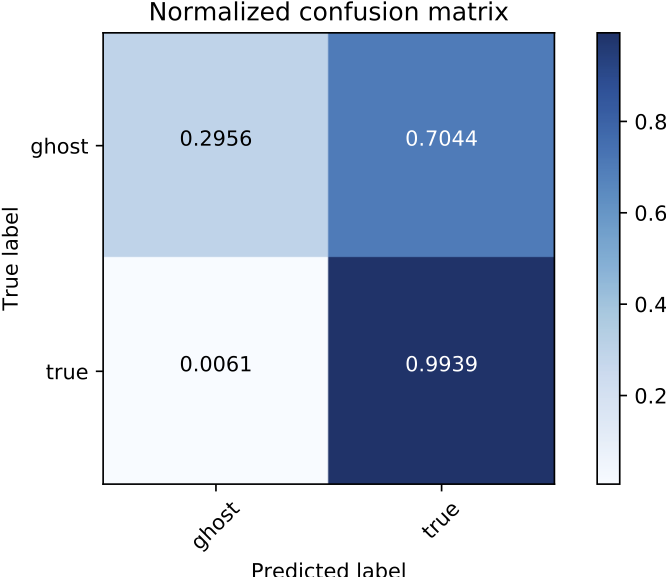
\includegraphics[scale=0.6]{figures/bBDT_normalized_cm.png}
\caption{Normalised confusion matrix determined for the trained bonsai BDT (binned) model.}
\label{fig:CM normalized}
\end{figure}

\section{T-Seed classifier: studies based on the deep neural networks}

The final model that was taken into consideration when working on a T-Seed selection model was deep neural network, described in \ref{sec:DNN}. 
All described studies were conducted using PyTorch framework \cite{pytorch}, which allows performing tensor computation acceleration via graphics processing units (GPU) and supports automatic differentiation. Moreover, Pytorch supports the C++ interface, which makes the model's deployment within the LHCb trigger convenient. 
However, studies discussed in this section were never deployed within the LHCb trigger system due to the algorithm's submission deadline \footnote{I am not sure if I should mention this.}, and the model based on bonsai Boosted Decision Trees was selected instead.  Nevertheless, the author decided to include this section since it may be useful for future studies. 
 
Pytorch provides a number of utility classes that abstract a lot of complexity, such as data parallelization and batching. From a practical perspective, the developer needs to ensure a customized implementation of the following classes: 

\begin{itemize}
\item \textbf{Dataset}. This class is dedicated to retrieving the input data,  applying data transformations and data argumentation logic, and converting processed data into the PyTorch tensor.  Within the scope of the presented study, the transformations were limited to adding such features as pseudorapidity and the data normalization. 
 \item \textbf{DataLoader}. The DataLoader combines a Datasets object with different samplers producing data batches. Samplers are an implementation of a different strategy for providing data to models. 
\item \textbf{Criterion}. The criterion is an abstraction of the loss function. Within this study's scope, only the Cross-entropy were used, although other options may be worth trying, see section \ref{sec:Focal_loss}. 
\item \textbf{Optimizer}. An optimizer is an object that holds the current state of the model and update parameters based on the computed gradients. The choice of the optimizer is considered as a model hyperparameter. However, the recommended and used in the presented studies choice is Adam. 
\item \textbf{Model}. It is an abstraction that defines the forward propagation, and it contains all components (layers) of the model.
Thus, the researcher has to implement two methods. The first one is the \textit{init} method, which initializes the network's layers. It is recommended to initialize the layers using the so-called Xavier initialization \cite{xavier}.  The second method that has to be implemented is the \textit{forward} method. It defines how the input tensor is processed in order to get a vector of output probabilities. The framework takes care of the backward propagation, so the researcher does not need to manually calculate the gradients of the loss function. 
\item \textbf{Training loop}. This utility function defines the way how the model is trained and allows customizing training progress measurement. 
Roughly speaking, the training loop consists of two nested loops (one over epochs and the second one over batches of data). 
Within the presented studies' scope, the training progress was measured as loss function versus epoch and batch. To ensure model implementation correctness, quantities such as information flow and the changes in the model's weight distributions over time were monitored. An exemplary plot of the information flow is shown in figure \ref{fig:gradient_flow}.
\end{itemize}

\begin{figure}[!h]
\centering
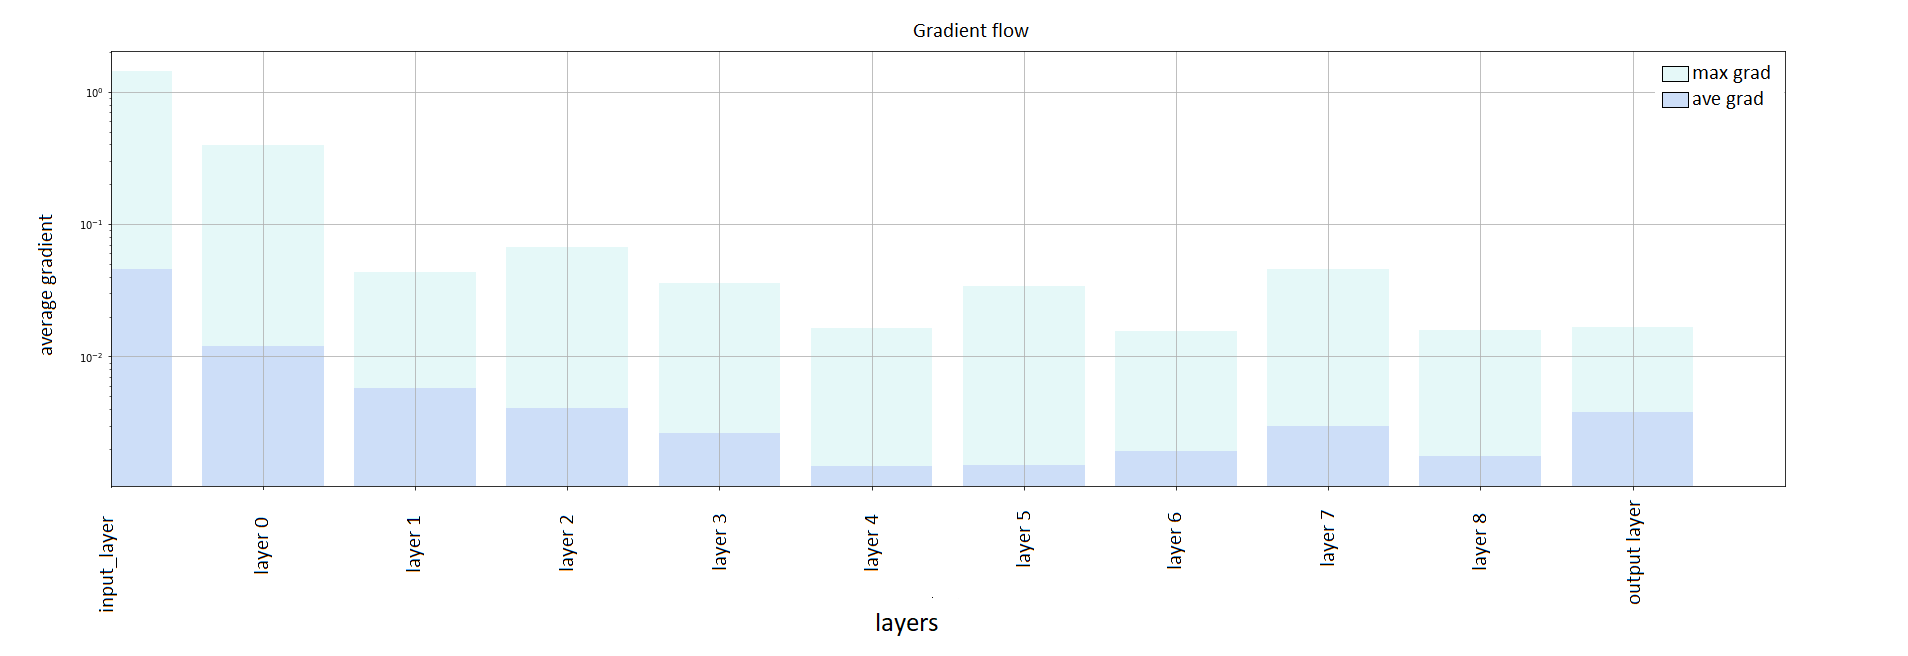
\includegraphics[width=\textwidth]{figures/NN/Gradient_flow.png}
\caption{Information or gradient flow visualization. This figure was generated for network with ten hidden units.The light blue bars indicate mean value of the information flow, while the dark blue bars represent maximum value of it.    
\label{fig:gradient_flow}}
\end{figure}


When all of the mentioned components are implemented, the next step is to check whether the model can overfit a small sample of the data, this method was recommended in \cite{karpathy}. If the model is not able to reach a low error rate that may indicate some issues, bugs, or misconfiguration.

The most time-consuming part of the study was the optimization of the network's architecture since the number of tested models exceeds one hundred, and training one model might take a couple of hours.

The architecture optimization procedure consists of the following steps. Start with a shallow network, that contains one hidden layer only.  Then iteratively extend the previously tested model by adding a hidden layer, which makes the model deeper.  Within each iteration step, try to optimize the architecture of the current network. The following options were considered: 

\begin{itemize}
\item Use the constant number of neurons per hidden layer; 
\item Build a triangle-type of a network, where the number of the hidden neurons decrease with network depth; 
\item Optimize number of hidden units per layer using Bayesian Optimization;
\item Use the Batch Normalization layer. This special layer normalizes the output of a previous activation layer by subtracting the batch mean and dividing by the batch standard deviation. For more details on how the Batch Normalization works, see \cite{batch_norm}. 
\item Use dropout layer. The dropout layer works by randomly setting the outgoing edges of hidden units (neurons that make up hidden layers) to zero at each update of the training phase. The detailed description of the dropout layer can be found in the original paper \cite{dropout}. 
\end{itemize}


\begin{figure}[!htb]
  \centering
\begin{tabular}{c c}
\subfloat{{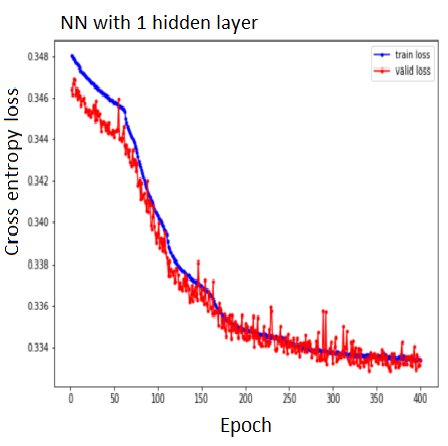
\includegraphics[width=0.4\textwidth]{figures/NN/learning_curve1nn.png} }}%
    \subfloat{{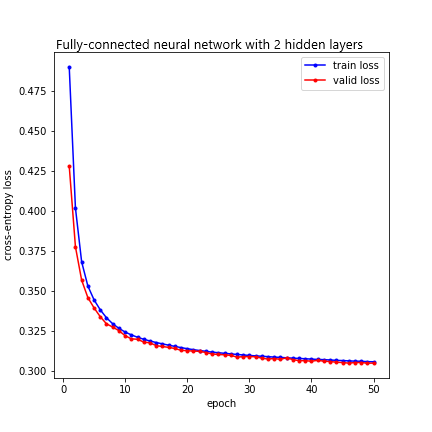
\includegraphics[width=0.4\textwidth]{figures/NN/learning_curve2nn.png} }}%
\\
\subfloat{{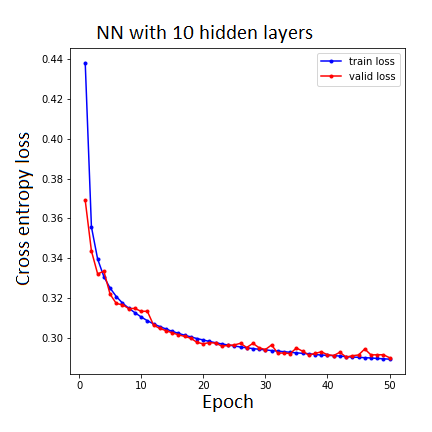
\includegraphics[width=0.4\textwidth]{figures/NN/learning_curve10nn.png}}}%
    \subfloat{{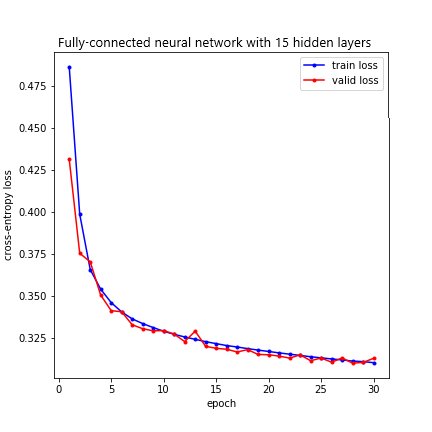
\includegraphics[width=0.4\textwidth]{figures/NN/learning_curve15nn.png} }}%
\end{tabular}
   \caption{Fully-connected neural network learning rates.  Each of the plot was obtained for model having different number of hidden layer. Upper left for one, upper right two, bottom left ten and  bottom right fifteen. 
\label{fig:DNN_learning_rates}}  
\end{figure}


Within the presented study, models with up to fifteen hidden layers were tested. Figure \ref{fig:DNN_learning_rates} presents a selected four learning curves (cross-entropy loss versus the number of training epoch) each of them documents training progress of a model with a different number of hidden layers. Surprisingly, adding more than two hidden layers to the model has a neglectable influence on the model prediction performance, even though the number of the network parameters was increased by two orders of magnitude.  Thus, the recommended architecture of the network contains two hidden layers. Such a shallow network 
produce similar results, measured as a ROC AUC, to the optimized xgboost one, which is shown in figure \ref{fig:DNN_roc}.

\begin{figure}[!ht]
\centering
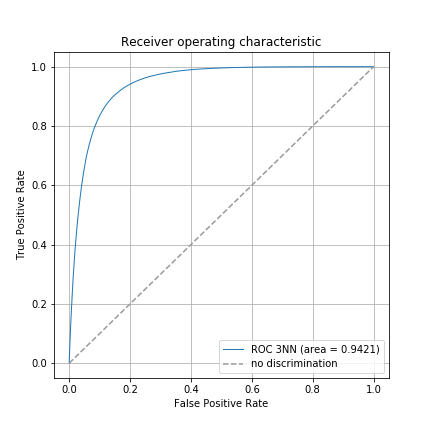
\includegraphics[scale=0.7]{figures/NN/roc_3nn.png}
\caption{ Fully-connected neural network containing two hidden layers ROC curve for selecting true T tracks using a simulated  $B_0\rightarrow J/\psi K_S^0 $ sample.      
\label{fig:DNN_roc}}
\end{figure}


\section{T-Seed classifier: model output interpretation}

This section is dedicated to emphasizing the importance of the model's interpretability. As presented before the T-Seed filter achieved satisfactory overall performance, but the question regarding the reliance still remains open.
Within the scope of this thesis, the three approaches to interpret Boosted Decision Tree model prediction have been tested, each of them has been described in section \ref{sec:lime}. 
The classical approach to interpret feature importance is to look at the model globally. The usual way to view the importance of the features is to investigate the following metrics: 

\begin{itemize}
    \item The feature \textbf{weight} is the number of times a feature appears in a tree across an ensemble of trees. For instance, if the model was built on top of the dataset consisting  of 100 entries, five features and the model itself consist of 3 trees, and suppose the \textit{feature1} occurs in the 1 splits, 2 splits, and 3 splits in each of three trees respectively, then the weight for \textit{feature1} will be $1+2+3=6$.   
    \item The \textbf{Gain} measures the relative contribution of the corresponding feature to model by taking each feature's contribution for each tree within the model. This metric can be interpreted as an average training loss reduction gained when using the feature for a split, in the other words is the improvement of the accuracy brought by a feature to the branches it is on. 
    \item The \textbf{Coverage} describes the relative number of observations related to this feature. In the above example if the \textit{feature1} is used to decide the leaf node for 20, 10, 5 observations in the mentioned trees respectively, then the coverage for this feature is $20+10+5 = 35$.   
\end{itemize}

Figure \ref{fig:xgboost overall features importance} presents three plots, each for different matrices described above. It is clearly visible, that these plots contradict to each other. According to the feature weights, the most important feature is seed $\chi^2\/dof$ and the $N_{hits}$ is redundant, while the coverage metric scores it as a second most important.

To understand why some, possibly categorical, feature has smaller weight value consider the following example. Let feature1 be a binary feature, which is highly correlated with the target variable and its inclusion or removal has a significant influence on classifier performance. Due to the nature of feature1, it has a tiny number of possible values compared to the other features. This feature can be used at most once per tree, while continues features may appear more often on a different level of the tree. Therefore, such a feature gets very low weight value. 

For the above reason, none of the presented global metrics gives an ultimate estimation of the importance of the feature. To get a better understating of it, taking into consideration the non-linear nature of the model's decision boundaries, it would be worth investigating different approaches of measuring the feature importance.  

\begin{figure}[!h]
\centering
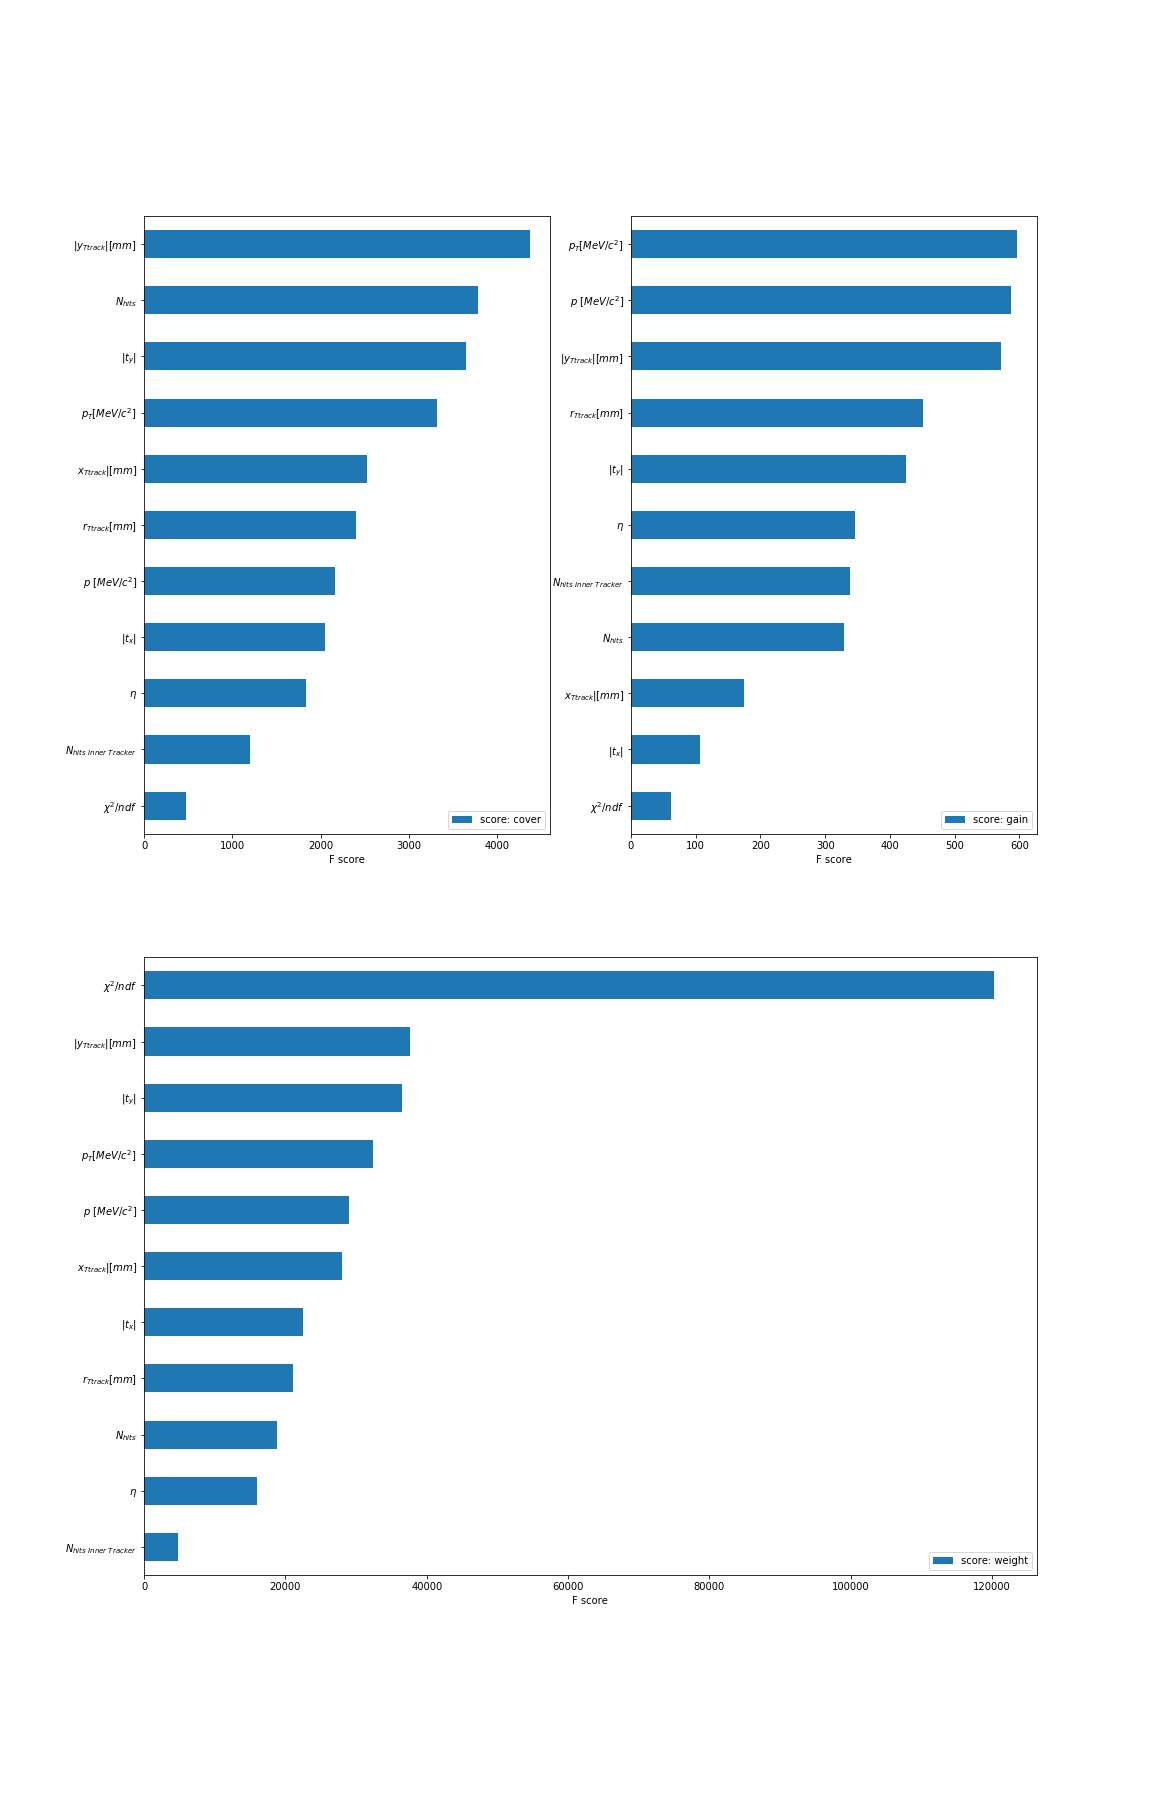
\includegraphics[scale=0.8]{figures/feature_importance.png}
\caption{Feature Importance plots for XGBoost model. Each of the plots were obtained for a different global feature importance metrics: coverage (upper left), gain (upper right) and weight (bottom). 
\label{fig:xgboost overal features importance}}
\end{figure}

The second method to take a closer look inside the xgboost black box is based on the idea of Shapley value, described in section [??]. The analysis of the importance of the features is usually done by presenting two groups of plots. The first group is presented in figure \ref{fig:shap overall}. The standardized importance plot provides a notion of relative feature importance and can be compared with the classical plots described previously. Although, it doesn't provide any additional information on the distribution of impacts that feature has on the model's output. This plot doesn't give any understanding of the feature's value on the model performance  \cite{Shap2}. To overcome this limitation the Shap summary plot was introduced, which leverages individualized feature attribution to the model's decision. In order to make that kind of plot the features are sorted by their global impact $\sum_{j=1}^{N}|\phi_i^{(j)}|$, then each of the dots corresponding to the Shap values $\phi_i^{(j)}|$ are plotted horizontally, stacked vertically when running out of space. This concept allows achieving similar effect to the violin plots, which can be further enhanced by coloring the dots according to the feature's value. 

\begin{figure}
\begin{tabular}{c}
\subfloat{{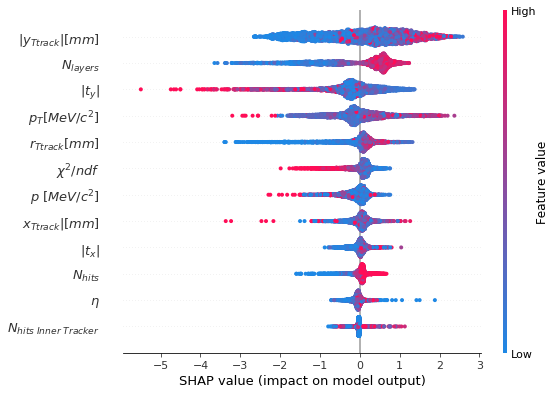
\includegraphics[width=\textwidth]{figures/Shap_overall.png} }}%
\\
\subfloat{{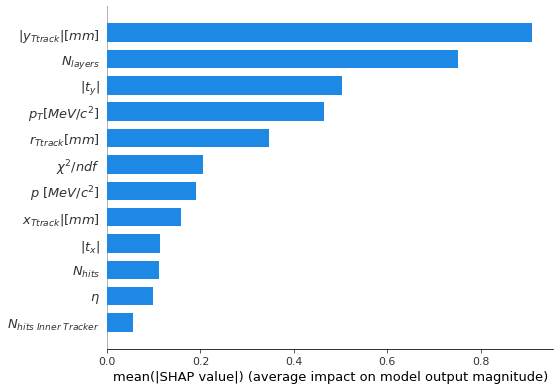
\includegraphics[width=\textwidth]{figures/Shap_mean.png}}}%
\end{tabular}
   \caption{Shap summary plots of all T-Seed classifier features. The plots were obtained using a sample of 50 thousand test examples. The interpretation of this plot is straightforward, the higher Shap value of the feature, the higher influence on the decision of whether T-Seed is reconstructable. In the upper plot, each dot represents every feature for every individual test example that was run through the model. Dot's are colored by the feature's value (red high, blue low). The bottom plot presents the standard feature importance bar plot. The x-axis is essentially the average magnitude change in model output when a feature is hidden from the model.}  
\label{fig:shap overall}
\end{figure}


To get a better understanding of Shap values presented in the figure \ref{fig:shap overall} let focus on one feature - $N_{layers}$. It is the second most important feature to decide whether T-Seed is a ghost. The impact of this feature on a model's output varies smoothly as the value of the feature increases, which is indicated by the smooth color gradient. The long tail reaching the left means that the extreme values of these features can significantly increase the probability that this T-Seed is not a valid seed. This is consistent with priory intuition saying the seed, that was reconstructed using a small number of hits are more likely to be a ghost. 

The second type of Shap based plots is dependence plots presented in figure \ref{fig:shap dep}.  The concept is similar to the pair-plot, which are usually created in order to visualize dependencies between two features. The shap dependence plots also take into consideration the Shap values. The idea is to make a scatter plot, shap value versus feature value, and apply color scheme that is based on the value of the second feature.

The plot (a) is the one that is the easiest to interpret. It shows the shap value versus the number of layers. It is clearly visible that T tracks with the numbers of plates smaller than 15 push strongly the classifier toward negative decisions. This effect is escalated when the track has a big value of $\chi^2 /\ dof $. This means the classifier decision agreed with an initial understanding of the problem, the track that was reconstructed using a small number of hits and it's fit to the track model has a poor quality is more likely to be a ghost. 


\begin{figure}[!ht]
\begin{center}
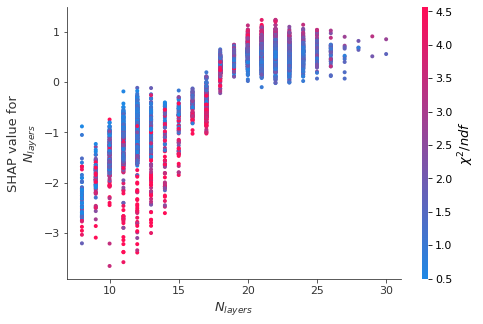
\includegraphics[width = 0.49\textwidth]{figures/dependence_plot3.png} 
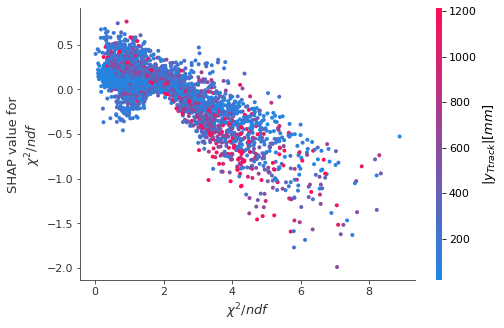
\includegraphics[width = 0.49\textwidth]{figures/dependence_plot1.png} \\
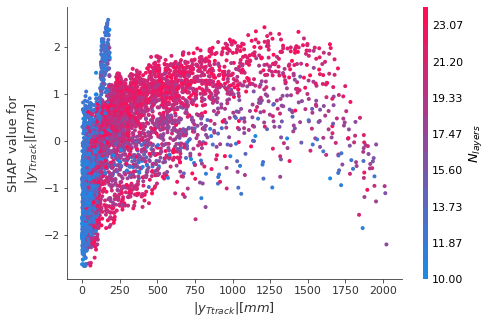
\includegraphics[width = 0.49\textwidth]{figures/dependence_plot2.png} 
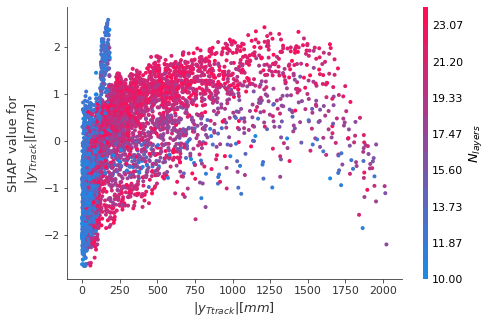
\includegraphics[ width = 0.49\textwidth]{figures/dependence_plot2.png} \\
   \caption{Shap dependence plots. Each dot is a track. The x-axis shows the value of the \textbf{feature 1} and the y-axis is the Shap value attributed to this feature. To show the dependence between \textbf{feature 1} and \textbf{feature 2} the color of particular dot depends of the value of the \textbf{feature 2}. }
   \label{fig:shap dep}
 \end{center}
 \end{figure}

The result of the evaluation of the third and final approach, the one that is base on LIME model, is shown in figure \ref{fig:limeResult}. The presented LIME outcome ware obtained for two randomly chosen test examples. Each of these examples represents one of the target classes. It provides a good indication of the importance of the features and highlights why particular decision was made. The length of each bar is proportional to the feature's value times linear regression weight associated with this feature.  It is easy to notice, that one of the most important feature is the number of hits, that were used to reconstruct T-Seeds and this is consistent with the initial intuition.  

\begin{figure}
\begin{subfigure}
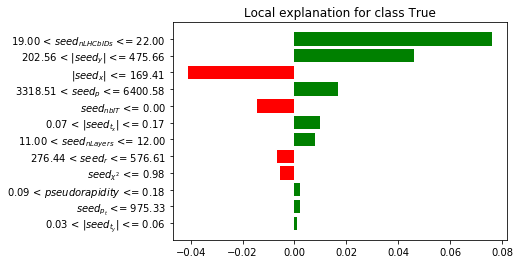
\includegraphics[width=\linewidth]{figures/LIME_true.png}
\caption{LIME explanation for randomly chosen True example  }
\end{subfigure}
\hfill
\begin{subfigure}
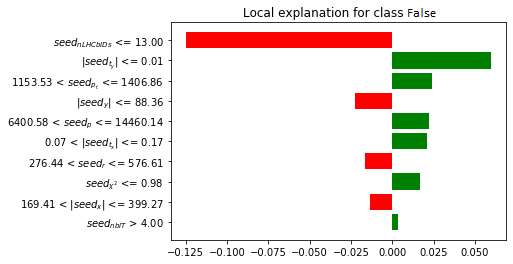
\includegraphics[width=\linewidth]{figures/lime_ghost.png}
\caption{LIME explanation for randomly chosen Ghost example}
\end{subfigure}%
\caption{Exemplary outcome of the LIME for two randomly chosen examples. Those samples were drown from the test dataset. 
The red color indicates that the features pushed prediction toward ghost. 
}\label{fig:limeResult}
\end{figure}




\section{Physics Performance of the modernised downstream tracking}
\label{sec:physic_performance}
The previous sections describe the LongLived pattern recognition algorithm. This one is dedicated to showing the physics performance of this algorithm. The performance can be measured using various strategies. The most obvious one is to measure the efficiency of reconstructing a charged particle in the acceptance as a downstream track using Monte Carlo simulated samples.
The second method uses to evaluate the performance using real data. This method determines and compares the pattern recognition algorithm performance by measuring the mass resolution.  

\subsection{Monte Carlo based Downstream Tracking efficiency  }

The pattern recognition algorithm performance measurement can be determined from Monte Carlo simulations by comparing the number of track that the algorithm managed to find (reconstructed tracks) with the maximum number of track that it could possibly find (reconstructable tracks). This section is based on the one \cite{PATLLT}. 

To discuss the efficiency of the pattern recognition algorithm it is obligatory to define a number of quantities that are used in this study.  First of all, the MC particle is said to be \textbf{reconstructible}, if it left the sufficient number of hits in the detector. The particle reconstructible criteria vary for one subdetector to another, and they are summarized \cite{track_def}:

\begin{itemize}
    \item Velo reconstructible is a particle that has at least three hits in $R$ and $\varphi$ sensors.
    \item TT reconstructible particle is consider when it has at least one hit in the first two planes (TTa) and one hit in the last tow planes (TTb). 
    \item T-Station reconstructible is a particle that has at least one x and one stereo hit in each of the three T-Stations. 
\end{itemize}

Therefore the definition of particle reconstructible as a Downstream track if it satisfies the TT and T-Stations reconstructibility criteria. In order to associate the reconstructed tracks to the reconstructable ones a cross-check of hits in both of them has to be evaluated. A reconstructed track is considered as matched to a simulated Monte Carlo particle if they share at least 70\% of the hits.  
Based on this definition the following pattern recognition performance metrics can be defined: 

\begin{itemize}
    \item The \textbf{Tracking efficiency} ($\varepsilon$) is defined as a ratio between the amount od reconstructed and matched track to the total amount of reconstructable tracks. 
    \begin{equation}
        \varepsilon  = \frac{\textrm{reconstructed} \cap  \textrm{matched}}{\textrm{reconstructable}}
    \end{equation}
    \item The \textbf{ghost rate} is the amount of reconstructed tracks not associated to any of the Monte Carlo particle, thus having less than 70\% of matched hits, with respect to the total amount of tracks found by the pattern recognition algorithm
    \begin{equation}
       \textrm{ghost rate} =  \frac{\textrm{not matched}}{\textrm{reconstructable}}
    \end{equation}
\end{itemize}

 Within the scope of this analysis the efficiency of a Downstream Tracking algorithm is calculated as the one that includes the efficiency of a Long-Lived Tracking pattern recognition algorithm combined together with the efficiency of the T-Seed reconstruction.

In the presented studies, the analysis was performed on a sample constituted of 50,000 simulated events of both magnet polarities. Two types of decays were simulated: $B^{0} \rightarrow J/\Psi K^{0}_{S}$ and $D^{*+} \rightarrow D^{0}\pi^+$. The first type of decay was selected to represent $B$ meson decays and the second one for a charm. 
There are four different categories of track that were considered within the scope of this performance analysis on MC data:

\begin{itemize}
    \item $\varepsilon_{TT+T}$ : efficiency for all downstream reconstructible particles;
    \item $\varepsilon_{TT+T, p>5Gev/c}$ : efficiency for all downstream reconstructible particles with $p> 5 GeV/c$;
    \item $\varepsilon_{TT+T, from B/D}$ : efficiency for all downstream reconstructible particles from a decay of $B$ or $D$ meson;
    \item $\varepsilon_{TT+T, from B/D, p>5 GeV }$ : efficiency for all downstream reconstructible particles from a decay of $B$ or $D$ meson with  $p> 5 GeV/c$.;
\end{itemize}

The overall efficiency numbers are collected in upper half of Table \ref{table:overall eff} and the ghost rate related numbers are presented in \ref{tab:overall ghost} (upper half). Plots of the efficiency and the ghost rate as a function of momentum, transverse momentum, and pseudorapidity are shown in 
figures \ref{fig:EffPatLLTBJpsiK}, \ref{fig:ghostPatLLTBJpsiK}  (obtained using  $B^{0} \rightarrow J/\Psi K^{0}_{S}$ ) and \ref{fig:EffPatLLTDstD0pi}, \ref{fig:ghostsPatLLTDstD0pi} (for $D^{*+} \rightarrow D^{0}\pi^+$ decay). No uncertainty is given, because presented numbers were obtained on a Monte Carlo samples not on a collision data. The statistical uncertainty are negligible, at the permille level.  

It was also important to measure the downstream tracking efficiency using the samples that were fitted with Kalman Filter and a quality cut on a $\chi^2\/ndf$ was applied. Those tracks were also proceeded by a clone killing algorithm to remove duplicates, which were reconstructed as long and downstream track simultaneously. The performance numbers referring to those tracks are collected in Table \ref{tab:overall eff}, lower half, and Table \ref{tab:overall ghost} (lower half) gives ghost rates. The performance numbers after these three steps seem worse than before, as the processing steps applied also reject correct tracks, and the cloned killer is inefficient. One of the reasons why it happens, the clon killer sometimes falsely classifies downstream tracks as long
tracks (for example when the Velo part is a ghost), which then gets removed from the downstream statistics. Furthermore, clone killing prefers long tracks over downstream tracks. 

Downstream tracking efficiency strongly depends on the momentum and transverse momentum of the tracks. The explanation of the phenomenon can be based on factors such as the search windows do not cover the full region necessary to find all tracks. Secondly, for low momentum tracks, search windows are generally larger than for high momentum tracks, which increases the number of hits in the search window, and increases the chances that the pattern recognition identifies the wrong hits.

In addition, the downstream tracks that were also reconstructed as long tracks
are less prone to be ghosts, which is why the ghost fraction actually increases
after the Kalman Filter, the clone killer and the ghost probability cut. However, it should be noted that
in a physics analysis of a decay channel, a strict cut is normally placed on the ghost probability of the downstream tracks, which reduces the ghost fraction
significantly.


\begin{table}[htp]
\caption{Reconstruction efficiency of downstream tracks on simulated samples of
$B^{0} \rightarrow J/\Psi K^{0}_{S}$ and $D^{*+} \rightarrow D^{0}\pi^+$ decays. The upper half are non-filtered tracks, the lower half is after the clone killer, Kalman Filter and ghost probability. This efficiency
includes the efficiency of T-Seed reconstruction and LongLived Tracking. Due to a softer
momentum spectrum, the efficiency is lower in the$D^{*+} \rightarrow D^{0}\pi^+$
sample.}
\begin{center}
\begin{tabular}{c|c|c|c|c|c}
filter & decay type & $\varepsilon_{TT+T}$ & $\varepsilon_{TT+T, ~p>5 GeV}$ & $\varepsilon_{TT+T\text{, from} B/D}$ & $\varepsilon_{TT+T\text{, from} B/D, ~p>5 GeV}$ \\
\hline
No &$B^{0} \rightarrow J/\Psi K^{0}_{S}$  & 73.3\% & 80.1\% & 81.4\% & 85.4\%\\
No &  $D^{*+} \rightarrow D^{0}\pi^+$ & 71.3\% & 78.0\% & 76.8\% & 81.4\% \\
\hline
Yes & $B^{0} \rightarrow J/\Psi K^{0}_{S}$  & 70.0\% & 76.7\% & 79.0\% & 83.2\% \\
Yes & $D^{*+} \rightarrow D^{0}\pi^+$ & 67.3\% & 73.7\% & 73.1\% & 77.3\%
\end{tabular}
\end{center}
\label{tab:overall eff}
\end{table}%

%%%%%%%%%%%%%%%%%%%%%%%%%%%%%%%%%%%%%%%%%%%%%%%%%%%%%%%%%%
\begin{table}[htp]
\caption{Ghost fraction of downstream tracks on simulated samples of
$B^{0} \rightarrow J/\Psi K^{0}_{S}$ and $D^{*+} \rightarrow D^{0}\pi^+$ decays. The upper half are non-filtered tracks, the lower half is after the clone killer, Kalman Filter and ghost probability. This ghost fraction
includes the ghosts produced in T-Seed pattern Recognition and Long-Lived Tracking. Due to a
softer momentum spectrum, the ghost fraction is higher in the
 $D^{*+} \rightarrow D^{0}\pi^+$ sample.}
\begin{center}
\begin{tabular}{c|c|c}
filter & decay type & fraction of ghosts \\
\hline
No & $B^{0} \rightarrow J/\Psi K^{0}_{S}$ & 29.5\% \\
No & $D^{*+} \rightarrow D^{0}\pi^+$ & 30.3\% \\
\hline
yes &$B^{0} \rightarrow J/\Psi K^{0}_{S}$ & 39.2\% \\
yes & $D^{*+} \rightarrow D^{0}\pi^+$ & 40.2\% \\
\end{tabular}
\end{center}
\label{tab:overall ghost}
\end{table}%



\begin{figure}[tbph]
\begin{center}
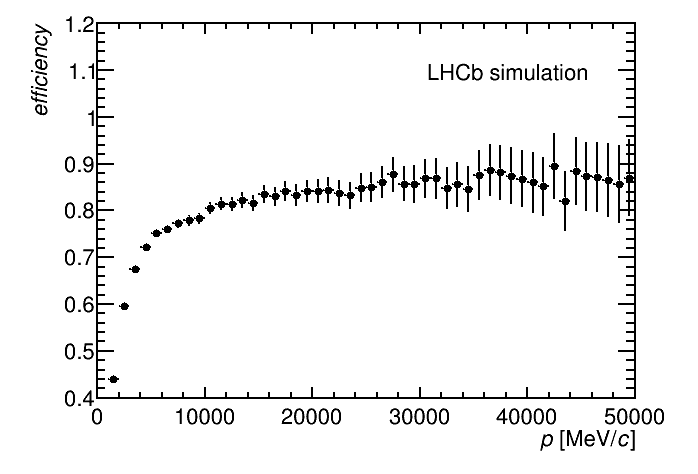
\includegraphics[width = 0.49\textwidth]{figures/EffPatLLT/overall/BJpsiKSP.png}
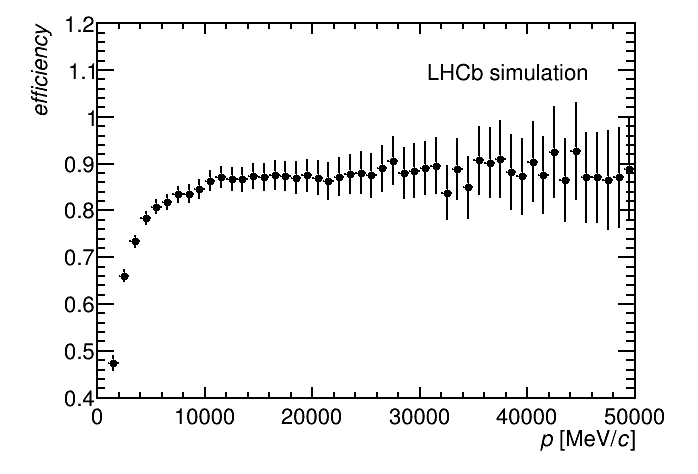
\includegraphics[width = 0.49\textwidth]{figures/EffPatLLT/overall/BJpsiKSFromBDP.png}
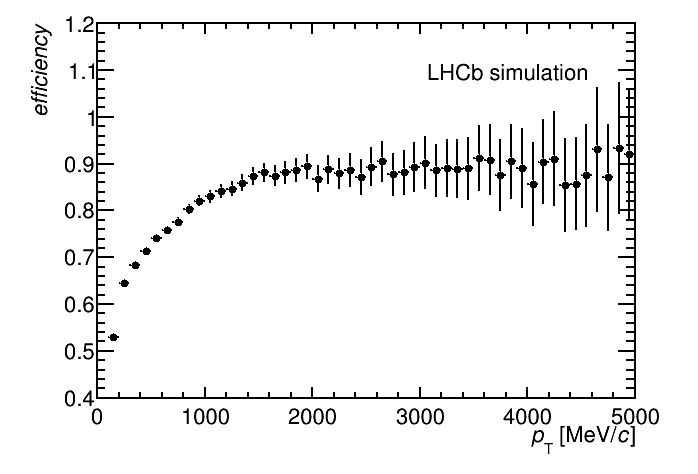
\includegraphics[width = 0.49\textwidth]{figures/EffPatLLT/overall/BJpsiKSPt.png}
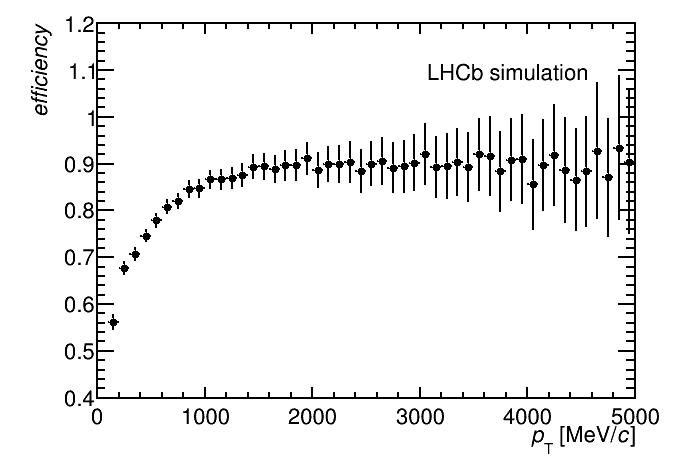
\includegraphics[width = 0.49\textwidth]{figures/EffPatLLT/overall/BJpsiKSFromBDPt.png}
\includegraphics[width = 0.49\textwidth]{figures/EffPatLLT/overall/BJpsiKSEta.png}
\includegraphics[width = 0.49\textwidth]{figures/EffPatLLT/overall/BJpsiKSFromBDEta.png}
\caption{Efficiencies to reconstruct downstream tracks as a function of momentum
(top row), transverse momentum (middle row) and pseudorapidity (bottom row). The
left column is for all downstream reconstructible tracks, the right column for
all downstream tracks from a decay chain of a $B$ or $D$ meson. The efficiencies are
obtained on a simulated sample of  $B^{0} \rightarrow J/\Psi K^{0}_{S}$ decays.}
\label{fig:EffPatLLTBJpsiK}
 \end{center}
\end{figure}
%%%%%%%%%%%%%%%%%%%%%%%%%%%%%%%%%%%%%%%%%%%%%%%%%%%%%%%%%%
\begin{figure}[tbph]
\begin{center}
\includegraphics[width = 0.49\textwidth]{figures/EffPatLLT/overall/BJpsiKSGhostFracP.png}
\includegraphics[width = 0.49\textwidth]{figures/EffPatLLT/overall/BJpsiKSGhostFracPt.png}
\includegraphics[width = 0.49\textwidth]{figures/EffPatLLT/overall/BJpsiKSGhostFracEta.png}
\caption{Ghost fraction in downstream tracks as a function of momentum (top
left), transverse momentum (top right) and pseudorapidity (bottom). The ghost
fractions are obtained on a simulated sample of  $B^{0} \rightarrow J/\Psi K^{0}_{S}$ decays.}
\label{fig:ghostPatLLTBJpsiK}
 \end{center}
 \end{figure}
%%%%%%%%%%%%%%%%%%%%%%%%%%%%%%%%%%%%%%%%%%%%%%%%%%%%%%%%%%
\begin{figure}[tbph]
\begin{center}
\includegraphics[width = 0.49\textwidth]{figures/EffPatLLT/overall/BJpsiKSP_TBTC.png}
\includegraphics[width = 0.49\textwidth]{figures/EffPatLLT/overall/BJpsiKSFromBDP_TBTC.png}
\includegraphics[width = 0.49\textwidth]{figures/EffPatLLT/overall/BJpsiKSPt_TBTC.png}
\includegraphics[width = 0.49\textwidth]{figures/EffPatLLT/overall/BJpsiKSFromBDPt_TBTC.png}
\includegraphics[width = 0.49\textwidth]{figures/EffPatLLT/overall/BJpsiKSEta_TBTC.png}
\includegraphics[width = 0.49\textwidth]{figures/EffPatLLT/overall/BJpsiKSFromBDEta_TBTC.png}
\caption{Efficiencies to reconstruct downstream tracks, after clone killing,
Kalman filtering and the cut on the ghost probability, as a function of momentum
(top row), transverse momentum (middle row) and pseudorapidity (bottom row). The
left column is for all downstream reconstructible tracks, the right column for
all downstream tracks from a decay chain of a $B$ or $D$ meson. The efficiencies are
obtained on a simulated sample of  $B^{0} \rightarrow J/\Psi K^{0}_{S}$ decays.}
\label{fig:EffPatLLTBJpsiK_TBTC}
 \end{center}
 \end{figure}
%%%%%%%%%%%%%%%%%%%%%%%%%%%%%%%%%%%%%%%%%%%%%%%%%%%%%%%%%%
\begin{figure}[tbph]
\begin{center}
\includegraphics[width = 0.49\textwidth]{figures/EffPatLLT/overall/BJpsiKSGhostFracP_TBTC.png}
\includegraphics[width = 0.49\textwidth]{figures/EffPatLLT/overall/BJpsiKSGhostFracPt_TBTC.png}
\includegraphics[width = 0.49\textwidth]{figures/EffPatLLT/overall/BJpsiKSGhostFracEta_TBTC.png}
\caption{Ghost fraction in downstream tracks, after clone killing, Kalman
filtering and the cut on the ghost probability, as a function of momentum (top
left), transverse momentum (top right) and pseudorapidity (bottom). The ghost
fractions are obtained on a simulated sample of $B^{0} \rightarrow J/\Psi K^{0}_{S}$ decays.}
\label{fig:ghostPatLLTBJpsiK_TBTC}
 \end{center}
 \end{figure}


\begin{figure}[tbph]
\begin{center}
\includegraphics[width = 0.49\textwidth]{figures/EffPatLLT/overall/DstD0piP.png} 
\includegraphics[width = 0.49\textwidth]{figures/EffPatLLT/overall/DstD0piFromBDP.png}
\includegraphics[width = 0.49\textwidth]{figures/EffPatLLT/overall/DstD0piPt.png} 
\includegraphics[width = 0.49\textwidth]{figures/EffPatLLT/overall/DstD0piFromBDPt.png}
\includegraphics[width = 0.49\textwidth]{figures/EffPatLLT/overall/DstD0piEta.png} 
\includegraphics[width = 0.49\textwidth]{figures/EffPatLLT/overall/DstD0piFromBDEta.png}
\caption{Efficiencies to reconstruct downstream tracks as a function of momentum (top row), transverse momentum (middle row) and pseudorapidity (bottom row). The left column is for all downstream reconstructible tracks, the right column for all downstream tracks from a decay chain of a $B$ or $D$ meson. The efficiencies are obtained on a simulated sample of$D^{*+} \rightarrow D^{0}\pi^+$ decays.}
\label{fig:EffPatLLTDstD0pi}
 \end{center}
 \end{figure}

\begin{figure}[tbph]
\begin{center}
\includegraphics[width = 0.49\textwidth]{figures/EffPatLLT/overall/DstD0piP_TBTC.png} 
\includegraphics[width =0.49\textwidth]{figures/EffPatLLT/overall/DstD0piFromBDP_TBTC.png}
\includegraphics[width = 0.49\textwidth]{figures/EffPatLLT/overall/DstD0piPt_TBTC.png} 
\includegraphics[width =0.49\textwidth]{figures/EffPatLLT/overall/DstD0piFromBDPt_TBTC.png}
\includegraphics[width = 0.49\textwidth]{figures/EffPatLLT/overall/DstD0piEta_TBTC.png} 
\includegraphics[width =0.49\textwidth]{figures/EffPatLLT/overall/DstD0piFromBDEta_TBTC.png}
\caption{Efficiencies to reconstruct downstream tracks, after clone killing, Kalman filtering and the cut on the ghost probability, as a function of momentum (top row), transverse momentum (middle row) and pseudorapidity (bottom row). The left column is for all downstream reconstructible tracks, the right column for all downstream tracks from a decay chain of a $B$ or $D$ meson. The efficiencies are obtained on a simulated sample of $D^{*+} \rightarrow D^{0}\pi^+$ decays.}
\label{fig:EffPatLLTDstD0p_TBTCi}
 \end{center}
 \end{figure}

\begin{figure}[tbph]
\begin{center}
\includegraphics[width=0.49\textwidth]{figures/EffPatLLT/overall/DstD0piGhostFracP.png} 
\includegraphics[width=0.49\textwidth]{figures/EffPatLLT/overall/DstD0piGhostFracPt.png}
\includegraphics[width=0.49\textwidth]{figures/EffPatLLT/overall/DstD0piGhostFracEta.png} 
\caption{Ghost fraction in downstream tracks as a function of momentum (top left), transverse momentum (top right) and pseudorapidity (bottom). The ghost fractions are obtained on a simulated sample of $D^{*+} \rightarrow D^{0}\pi^+$ decays.}
\label{fig:ghostsPatLLTDstD0pi}
 \end{center}
 \end{figure}

\begin{figure}[tbph]
\begin{center}
\includegraphics[width =0.49\textwidth]{figures/EffPatLLT/overall/DstD0piGhostFracP_TBTC.png} 
\includegraphics[width =0.49\textwidth]{figures/EffPatLLT/overall/DstD0piGhostFracPt_TBTC.png}
\includegraphics[width =0.49\textwidth]{figures/EffPatLLT/overall/DstD0piGhostFracEta_TBTC.png} 
\caption{Ghost fraction in downstream tracks, after clone killing, Kalman filtering and the cut on the ghost probability, as a function of momentum (top left), transverse momentum (top right) and pseudorapidity (bottom). The ghost fractions are obtained on a simulated sample of $D^{*+} \rightarrow D^{0}\pi^+$ decays.}
\label{fig:ghostsPatLLTDstD0pi_TBTC}
 \end{center}
 \end{figure}


\subsection{Comparison between Long-Lived Tracking algorithm and its predecessor}
The analysis presented within this section is dedicated to comparing the performance of the Long-Lived Tracking algorithm and its predecessor called PatDownstream \cite{PatDownstream}. The corresponding performance numbers are given in tables \ref{tab:PatLLTPatDownstreamEffComp} \ref{tab:PatLLTPatDownstreamEffCompTBTC} \ref{tab:globGhostComp}. 

Figures \ref{} \ref{ } show the efficiency and ghost rates of downstream tracks reconstructed via these two algorithms as a function of momentum, transverse momentum, and pseudorapidity. Those plots visualize tracking algorithm performance that was obtained using a simulated sample of B  and no other processing was applied. 

Figures \ref{} \ref{} present the same quantities, after Kalman filtering and clone killer. 
It is clearly visible, that the performance gain and the strong reduction of ghost rates were measured for the new algorithm. It is presumed that the significant ghost rate reduction (about 16\%) was achieved due to the good performance of the T-Seed classifier, which was one of the major goals of the author’s study. 


\begin{table}[htp]
\caption{Comparions of reconstruction efficiency of downstream tracks made with Long-Lived Tracking algorithm or PatDownstream, on simulated samples of $B^{0} \rightarrow J/\Psi K^{0}_{S}$ . This efficiency includes the efficiency of PatSeeding and Long-Lived Tracking algorithm.}
\begin{center}
\begin{tabular}{c|c|c|c|c}
algorithm & $\varepsilon_{TT+T}$ & $\varepsilon_{TT+T, ~p>5 GeV}$ & $\varepsilon_{TT+T\text{, from} B/D}$ & $\varepsilon_{TT+T\text{, from} B/D, ~p>5 GeV}$ \\
\hline 
Long-Lived Tracking & 73.3\% & 80.1\% & 81.4\% & 85.4\%\\
PatDownstream          & 68.3\% & 74.4\% & 77.1\% & 81.6\% 
\end{tabular}
\end{center}
\label{tab:PatLLTPatDownstreamEffComp}
\end{table}%

\begin{table}[htp]
\caption{Comparions of reconstruction efficiency of downstream tracks made with PatLongLivedTracking or PatDownstream, on simulated samples of $B^{0} \rightarrow J/\Psi K^{0}_{S}$, after the Kalman Filter and clone killer. This efficiency includes the efficiency of PatSeeding and PatLongLivedTracking. The efficiency decreases compared to Table~\ref{tab:PatLLTPatDownstreamEffComp} due to inefficiency of the clone killer.}
\begin{center}
\begin{tabular}{c|c|c|c|c}
algorithm & $\varepsilon_{TT+T}$ & $\varepsilon_{TT+T, ~p>5 GeV}$ & $\varepsilon_{TT+T\text{, from} B/D}$ & $\varepsilon_{TT+T\text{, from} B/D, ~p>5 GeV}$ \\
\hline 
Long-Lived Tracking & 70.0\% & 76.7\% & 79.0\% & 83.2\% \\
PatDownstream          & 63.7\% & 71.3\% & 74.5\% & 79.2\% 
\end{tabular}
\end{center}
\label{tab:PatLLTPatDownstreamEffCompTBTC}
\end{table}%

\begin{table}[htp]
\caption{Ghost fraction of downstream tracks on simulated samples of $B^{0} \rightarrow J/\Psi K^{0}_{S}$ for PatLongLivedTracking and PatDownstream, once before and after the clone killer, Kalman Filter and ghost probability (CKG) were applied. This ghost fraction includes the ghosts produced in PatSeeding and PatLongLivedTracking (PatDownstream). The ghost fraction is higher after the clone killer as tracks, also reconstructed as long tracks, are not present in that number.}
\begin{center}
\begin{tabular}{c|c|c}
algorithm & fraction of ghosts & fraction of ghosts after CKG \\
\hline 
Long-Lived Tracking & 29.5\% & 39.2\%\\
PatDownstream & 46.3\% & 52.1\% \\
\end{tabular}
\end{center}
\label{tab:globGhostComp}
\end{table}%



%%%%%%%%%%%%%%%%%%%%%%%%%%%%%%%%%%%%%%

\begin{figure}[tbph]
\begin{center}
\includegraphics[width = 0.49\textwidth]{figures/EffPatLLT/compare/BJpsiKSP.png} 
\includegraphics[width = 0.49\textwidth]{figures/EffPatLLT/compare/BJpsiKSFromBDP.png}
\includegraphics[width = 0.49\textwidth]{figures/EffPatLLT/compare/BJpsiKSPt.png} 
\includegraphics[width = 0.49\textwidth]{figures/EffPatLLT/compare/BJpsiKSFromBDPt.png}
\includegraphics[width = 0.49\textwidth]{figures/EffPatLLT/compare/BJpsiKSEta.png} 
\includegraphics[width = 0.49\textwidth]{figures/EffPatLLT/compare/BJpsiKSFromBDEta.png}
\caption{Efficiencies to reconstruct downstream tracks as a function of momentum (top row), transverse momentum (middle row) and pseudorapidity (bottom row), in red for Long-Lived Tracking algorithm and in black for PatDownstream. The left column is for all downstream reconstructible tracks, the right column for all downstream tracks from a decay chain of a $B$ or $D$ meson. The efficiencies are obtained on a simulated sample of  $B^{0} \rightarrow J/\Psi K^{0}_{S}$ decays.}
\label{fig:EffCompPatLLTBJpsiK}
 \end{center}
 \end{figure}

\begin{figure}[tbph]
\begin{center}
\includegraphics[width = 0.49\textwidth]{figures/EffPatLLT/compare/BJpsiKSGhostFracP.png} 
\includegraphics[width = 0.49\textwidth]{figures/EffPatLLT/compare/BJpsiKSGhostFracPt.png}
\includegraphics[width = 0.49\textwidth]{figures/EffPatLLT/compare/BJpsiKSGhostFracEta.png} 
\caption{Ghost fraction in downstream tracks as a function of momentum (top left), transverse momentum (top right) and pseudorapidity (bottom), in red for Long-Lived Tracking algorithm and in black for PatDownstream. The ghost fractions are obtained on a simulated sample of $B^{0} \rightarrow J/\Psi K^{0}_{S}$ decays.}
\label{fig:ghostCompPatLLTBJpsiK}
 \end{center}
 \end{figure}

%%%%%%%%%%%%%%
%%%%%%%%%%%%%%

\begin{figure}[tbph]
\begin{center}
\includegraphics[width = 0.49\textwidth]{figures/EffPatLLT/compare/BJpsiKSP_TBTC.png} 
\includegraphics[width = 0.49\textwidth]{figures/EffPatLLT/compare/BJpsiKSFromBDP_TBTC.png}
\includegraphics[width = 0.49\textwidth]{figures/EffPatLLT/compare/BJpsiKSPt_TBTC.png} 
\includegraphics[width = 0.49\textwidth]{figures/EffPatLLT/compare/BJpsiKSFromBDPt_TBTC.png}
\includegraphics[width = 0.49\textwidth]{figures/EffPatLLT/compare/BJpsiKSEta_TBTC.png} 
\includegraphics[width = 0.49\textwidth]{figures/EffPatLLT/compare/BJpsiKSFromBDEta_TBTC.png}
\caption{Efficiencies to reconstruct downstream tracks, after clone killing, Kalman filtering and the cut on the ghost probability, as a function of momentum (top row), transverse momentum (middle row) and pseudorapidity (bottom row). The left column is for all downstream reconstructible tracks, the right column for all downstream tracks from a decay chain of a $B$ or $D$ meson. The efficiencies are obtained on a simulated sample of  $B^{0} \rightarrow J/\Psi K^{0}_{S}$ decays.}
\label{fig:EffCompPatLLTBJpsiK_TBTC}
 \end{center}
 \end{figure}

\begin{figure}[tbph]
\begin{center}
\includegraphics[width = 0.49\textwidth]{figures/EffPatLLT/compare/BJpsiKSGhostFracP_TBTC.png} 
\includegraphics[width = 0.49\textwidth]{figures/EffPatLLT/compare/BJpsiKSGhostFracPt_TBTC.png}
\includegraphics[width = 0.49\textwidth]{figures/EffPatLLT/compare/BJpsiKSGhostFracEta_TBTC.png} 
\caption{Ghost fraction in downstream tracks, after clone killing, Kalman filtering and the cut on the ghost probability, as a function of momentum (top left), transverse momentum (top right) and pseudorapidity (bottom). The ghost fractions are obtained on a simulated sample of  $B^{0} \rightarrow J/\Psi K^{0}_{S}$ decays.}
\label{fig:ghostCompPatLLTBJpsiK_TBTC}
 \end{center}
 \end{figure}

\subsection{Performance measured using collision data}
\label{sec:performance_data}
The improvements that were performed on a pattern recognition algorithm should be reflected in improvements to the reconstruction of decayed particles. To investigate this, the reconstruction of $K_s$ and $\Lambda_0$ in minimum bias events \footnote{The minimum bias samples are those which try to reproduce proton-proton collisions as close to the reality as possible, with no bias from restricted trigger conditions.} were analyzed. 

\subsubsection{Event selection}

This analysis focuses on the algorithm's total event yield difference between the new algorithm and the baseline. Thus the selection was taken from the standard LHCB software, the following list contains an explanation of each cut applied to select the data that were used to reconstruct both $K_s$ and $\Lambda_{0}$:

\begin{itemize}
    \item \textbf{$p(\pi_1, \pi_2 \lor p)$} - minimal momentum of daughter particles;
    \item \textbf{$p_t(\pi_1, \pi_2 \lor p)$} - minimal transverse momentum of daughter particles;
    \item $\chi^2\/ndf$ of $\pi \lor p$ tracks - maximal  $\chi^2\/ndf$ of the daughter tracks;
    \item track type - the type of track that were taken into consideration;
    \item $\chi^2\/ndf$ $(K_S \lor \Lambda_0)$ - maximal $\chi^2\/ndf$ of the vertex fit;
    \item $\Delta M(\pi_1 + \pi_2 || p)$ - the difference between reconstructed invariant mass of the mother particle and its mass taken from the Particle Data Group (PDG) repository \cite{PDG}. This invariant mass is calculated by taking sum of 4-momenta vectors \footnote{4 vector is a generalization of the classical three-dimensional momentum vector to four-dimensional space-time. The covariant form of this vector can be written as: $p= (p^{0}, p^{1}, p^{2}, p^{3}) = (\frac{E}{c},p_x,p_y,p_z) $ }  of the two daughter particle tracks;   
    \item $\Delta M(K_S \lor \Lambda_0)$ -  the difference between reconstructed invariant mass and the PDG mass after vertex fit. The tracks has been properly propagated to the $K_s$ or $\Lambda_0$  vertex. 
\end{itemize}

 
\begin{table}[h]
\caption{Selection criteria for $K_s$ and $\Lambda_0$ }
\hspace*{1.2cm}
\begin{tabular}{|c|c|c|}
\hline
cut                                      & $K_S$              & $\Lambda_0$        \\ \hline
$p(\pi_1, \pi_2 \lor p)$ {[}MeV{]}              & \textgreater{}2000 & \textgreater{}2000 \\ \hline
$p_t(\pi_1, \pi_2 \lor p)$ {[}MeV{]}            & \textgreater{}50   & \textgreater{}100  \\ \hline
track type                               & Downstream         & Downstream         \\ \hline
$\chi^2\/ndf$ of $\pi \lor p$              & \textless{}4       & \textless{}4       \\ \hline
$\chi^2\/ndf$ $(K_S \lor \Lambda_0)$       & \textless{}10      & \textless{}10      \\ \hline
$\Delta M(\pi_1 + \pi_2 \lor p)$ {[}MeV{]} & \textless{}100     & \textless{}100     \\ \hline
$\Delta M(K_S \lor \Lambda_0)$ {[}MeV{]}   & \textless{}100     & \textless{}100     \\ \hline
\end{tabular}
\label{tab:cuts}
\end{table}
 
 
 The cuts for $K_s$ and $\Lambda_0$ are given in table \ref{tab:cuts}. The sample that was used to perform this analysis consist of about 100,000 events. Table \ref{tab:signal} presents signal yield of $K_s$ and $\Lambda_0$ and the background. In both cases, a significant increase in signal yield and background reduction is visible. Figures \ref{fig:Lambda_performance} and \ref{fig:Ks_performance} show the reconstructed invariant masses of a discussed particles. The model for mass distribution is a single Gaussian and an exponential background. Although a more complicated fit model would, in principle, be appropriate, e.g. a double Crystal Ball function, these fits were very unstable and showed problems converging. To avoid these complications and have a consistent mass model, a single Gaussian solution was chosen. As only ratios of event yields are considered, the error from using a single Gaussian only largely cancels. 
 

\begin{table}[h]
\centering
\caption{Signal yield and background of reconstructed $K_S$ and $\Lambda_0$ using minimum bias samples.  "Original" algorithm refers to the one before improvements, the "new" consists of two Machine Learning classifiers. }
\hspace*{-0.8cm}
\begin{tabular}{|c|c|c|c|c|c|}
\hline
version     & decay                               & signal                     & background                   & S/B ratio {[}\%{]} &  $\Delta$ signal [\%] \\ \hline 

original & $K_S^0 \rightarrow \pi^+ \pi^-$     & $2129 \pm 98$ & $14308 \pm 148$ & 14.9               & 0                           \\\hline 
new      & $K_S^0 \rightarrow \pi^+ \pi^-$     & $2194 \pm 96$ & $12872 \pm 141$ & 17                 & 3                           \\ \hline 
original & $\Lambda_0 \rightarrow p^+ \pi^-$ & $820\pm 44$                & $3316 \pm 67$   & 24.729             & 0                           \\ \hline 
new      & $\Lambda_0 \rightarrow p^+ \pi^-$ & $873 \pm 44$               & $3208 \pm 66 $  & 27.2               & 6.5   \\ \hline 
                    \end{tabular}
\label{tab:signal}
\end{table}

\begin{figure}[tbph]
\begin{center}
\includegraphics[width = 0.49\textwidth]{figures/tracking_ks/mass_lambda_baseline.png} 
\includegraphics[width = 0.49\textwidth]{figures/tracking_ks/mass_lambda_bdt.png}
\caption{Invariant mass distribution of reconstructed $\Lambda_0 \rightarrow p^{+} + \pi^{-}$ candidates.  The left plot present results generated using the baseline version of the Downstream tracking reconstruction algorithm and the right plot is a  similar graph for Long-Lived tracking algorithm. The red  dashed line is the signal modeled as a Gaussian distribution, the gray dashed line shows the background and the straight blue line shows the combination.}
\label{fig:Lambda_performance}
 \end{center}
 \end{figure}

\begin{figure}[tbph]
\begin{center}
\includegraphics[rotate=-90, width = 0.49\textwidth]{figures/tracking_ks/Mas_ks_baseline.pdf} 
\includegraphics[rotate=-90, width = 0.49\textwidth]{figures/tracking_ks/Mas_ks_bdt.pdf}
\caption{Invariant mass distribution of reconstructed $K_S \rightarrow \pi^{+} + \pi^{-}$ candidates.  The left plot present results generated using the baseline version of the Downstream tracking reconstruction algorithm and the right plot is a  similar graph for Long-Lived tracking algorithm. The red  dashed line is the signal modeled as a Gaussian distribution, the gray dashed line shows the background and the straight blue line shows the combination.}
\label{fig:Ks_performance}
 \end{center}
 \end{figure}




\subsection{Tuning of the Downstream tracking algorithm}

One of the key algorithm's parameters that has a strong influence on the pattern recognition performance is a T-Seed classification threshold. As described in section \ref{sec:hyperparameters}, its value was chosen to select more than 99\% of true T-seeds. This value corresponds to a very conservative classifier, which requires having extreme confidence to classify a given track as a ghost. As a result, the amount of suppressed background is reduced. Analyzing the ROC curve presented in figure \ref{fig:ROC binned}, one can conclude that devoting the tiny amount of signal data, the classifier can significantly reduce the background. This section is dedicated to fine-tuning the classification threshold. The presented analysis is based on measuring relative events yield for two channels, $K_s$ and $\Lambda_0$. The selection criteria were described in section \ref{sec:performance_data}. 

Table \ref{tab:finetuning} presents the results of fine-tuning procedure. Those numbers were taken from the $K_s$ and $\Lambda_0$ invariant mass fits, which are shown in figures \ref{fig:Lambda_finetuning} and \ref{fig:ks_finetuninh}. Each of the rows represents a different classification threshold value. It is clearly visible that increasing the value of T-Seed classification threshold parameter allows significantly reduces the background while preserving almost all signal events. One can conclude that increasing this value from 0.07 to 0.2 allows to suppress 18\% more background.  

To summarize this study, increasing the value of the classification threshold to 0.2 allows reducing the background of about \textbf{ 26\%} while keeping same number of signal events, measured in $K_s$ channel, with respect to the Long-Lived tracking predecessor. 

\begin{table}[h]
\caption{Evolution of the Long-Lived tracking algorithm $K_s$ and $\Lambda_0$ events yield for change of the T-Seed classification threshold.}
\hspace*{-2.5cm}
\begin{tabular}{|c|c|c|c|c|c|c|}
\hline
classification threshold & decay channel                                              & signal & background & S/B [\%] & $\Delta$ signal [\%] & $\Delta$ background [\%] \\ \hline
baseline 0.07            & \multirow{4}{*}{$K_S \rightarrow \pi^{+} + \pi^{-}$}       & 873    & 3208       & 27.21    & 0                    & 0                        \\ \cline{1-1} \cline{3-7} 
0.1                      &                                                            & 863    & 3081       & 28.01    & 1.1                  & 4                        \\ \cline{1-1} \cline{3-7} 
0.15                     &                                                            & 843    & 2920       & 28.87    & 3.4                  & 9                        \\ \cline{1-1} \cline{3-7} 
0.2                      &                                                            & 823    & 2747       & 29.96    & 5.7                  & 14.4                     \\ \hline
baseline 0.07            & \multirow{4}{*}{$\Lambda_0 \rightarrow \pi^{+} + \pi^{-}$} & 2194   & 12872      & 17.04    & 0                    & 0                        \\ \cline{1-1} \cline{3-7} 
0.1                      &                                                            & 2176   & 12220      & 17.81    & 0.8                  & 5.1                      \\ \cline{1-1} \cline{3-7} 
0.15                     &                                                            & 2152   & 11435      & 18.82    & 1.9                  & 11.2                     \\ \cline{1-1} \cline{3-7} 
0.2                      &                                                            & 2126   & 10542      & 20.17    & 3.1                  & 18.1                     \\ \hline
\end{tabular}
\label{tab:finetuning}
\end{table}


\begin{figure}[tbph]
\begin{center}
\includegraphics[rotate=-90, width = 0.49\textwidth]{figures/tracking_ks/Mass_lambda_bdt.pdf} 
\includegraphics[rotate=-90, width = 0.49\textwidth]{figures/tracking_ks/mas_labda_bdt_01.pdf} \\
\includegraphics[rotate=-90, width = 0.49\textwidth]{figures/tracking_ks/mas_labda_bdt_015.pdf}
\includegraphics[rotate=-90, width = 0.49\textwidth]{figures/tracking_ks/mas_labda_bdt_02.pdf}

\caption{Invariant mass distribution of reconstructed  $\Lambda_0 \rightarrow \pi^{+} + \pi^{-}$ candidates. Each plot corresponds to the different values of the T-Seed classifier threshold. The left upper plot presents  $Lambda_0$ invariant mass for a baseline (threshold =0.07), upper right corresponds to threshold = 0.1, and the lower plots threshold 0.15 and 0.2 (right and left respectively). The statistical uncertainties are correlated here because the identical sample is used }
\label{fig:Lambda_finetuning}
 \end{center}
 \end{figure}



\begin{figure}[tbph]
\begin{center}
\includegraphics[ rotate=-90, width = 0.49\textwidth]{figures/tracking_ks/Mas_ks_bdt.pdf} 
\includegraphics[rotate=-90, width = 0.49\textwidth]{figures/tracking_ks/Mas_ks_bdt_01.pdf} \\
\includegraphics[rotate=-90, width = 0.49\textwidth]{figures/tracking_ks/Mas_ks_bdt_015.pdf} 
\includegraphics[rotate=-90, width = 0.49\textwidth]{figures/tracking_ks/Mas_ks_bdt_02.pdf} \\
\caption{Invariant mass distribution of reconstructed  $K_S \rightarrow \pi^{+} + \pi^{-}$ candidates. Each plot corresponds to the different values of the T-Seed classifier threshold. The left upper plot presents  $\Lambda_0$ invariant mass for a baseline (threshold =0.07), upper right corresponds to threshold = 0.1, and the lower plots threshold 0.15 and 0.2 (right and left respectively). The statistical uncertainties are correlated here because the identical sample is used.}
\label{fig:ks_finetuninh}
 \end{center}
 \end{figure}
 

\subsection{Processing time}

As the Long-Lived Tracking algorithm processing time depends significantly on a type of machine, that is used to run it, and the event multiplicity it is hard to give an absolute unbiased number. On a simulated signal sample for Run II on a single worker node at CERN, Long-Lived Tracking needs $O(5 ms)$ to process an event. This time is not significant for the overall timing budget of HLT 2.
Comparisons using callgrind show a decrease in processing time compared to Long-Lived Trackig predecessor of about 45\%.

\section{Future work}
This section is dedicated to present ideas, that can be leverages to solve a similar types of problems and due to the LongLived Tracking algorithm's submission deadline were never implemented. One of the project that can benefit from those ideas is Downstream Tracking reconstruction for the Upgraded LHCb. 

That section contains a collection of concepts, that author would want to try or implement during the study on Downstream Tracking if he would have a time travel machine.

\subsection{Recurrent Neural Network}
The models that were implemented to classify seeds and select tracks candidates uses information about the entire tracks only. They don't utilize any information can be extracted from the hits that were used to reconstruct the input tracks.  



One possible enhancement to the Recurrent Neural Network is leveraging the idea of attention mechanism \cite{attention}.  Attention mechanism the method to provides an understanding of other relevant sequence elements into the one that is currently processing. In other words, it relates different positions of a single sequence in order to compute a representation of the sequence. Attention has been used successfully in a variety of tasks Natural Language Processing (NLP) and sequence modeling tasks

\subsection{Focal loss}
\label{sec:focal_loss}

The imbalanced classification problem occurs very often in the field of High Energy Physics. The distribution of the background examples significantly exceeds the number of interesting signal events. There are a number of methods on how to approach that kind of problem. Thus this section is dedicated to presenting the one based on a modification of a loss function. \footnote{The other method that is usually applied is dataset resampling.  The two main approaches to randomly resampling an imbalanced dataset are to delete examples from the majority class, called undersampling, and to duplicate examples from the minority class, called oversampling.}  The proposed loss function is called \textbf{focal loss} and given by \cite{focal_loss}: 

\begin{equation}
FL(p_t) = -(1-p_t)^{\gamma}log(p_t)
\end{equation}

where:

\begin{equation}
    p_t = \left\{ \begin{array}{ll}
p & \textrm{when $y$ is true}\\
1-p & \textrm{otherwise}\\
\end{array} \right.
\end{equation}
and $y$ specify the grand-true class and $p$ is a model's predicted probability for class with label $y=1$, and $\gamma$ is a hyperparameter that define how much the well classified examples are diminished.  Figure \ref{fig:Focal loss} presents the plot of the Focal loss versus probability of a true example being classified as a true one.

 \begin{figure}[!h]
\centering
\includegraphics{figures/Focal_loss.png}
\caption{Visualization of the Focal loss (FL) versus the probability of true class, obtained for a different value of hyperparameter $\gamma$. $\gamma=0$ corresponds to the cross-entropy. Figure taken from \cite{focal_loss}. 
\label{fig:Focal loss}}
\end{figure}


The idea of Focal loss was proposed to improve one stage image detection model. Image detection is a type of problem in which the model needs to find a location (bounding box) of particular objects, for instance, find a face on camera footage. In that kind of problem, the majority of regions are empty, and only a tiny number of them contain relevant objects. Thus this setup is very similar to the searching for an interesting physics signals. The Focal loss adds a factor $(1 - p_t)^\gamma$ to the standard cross-entropy criterion. Setting $\gamma > 0$ reduces the relative loss for well-classified examples ($p_t > 0.5$), putting more focus on hard, misclassified examples.
 
In order to use Focal Loss as an xgboost objective function, one needs to implement its first and second derivative. Which can be done manually or using one of the automatic derivation packages like Scipy \cite{scipy}.   

\subsection{Workflow Management System}

One of the parts of the study that can be enhanced is a pattern recognition validation and performance check. 
The current validation process requires a lot of manual intervention. The trained model needs to be extracted, then deployed within a Brunel application, after that Brunel output (DST file) is used as input to the DaVinci which produces Ntuple, which can be used by the custom root scripts to reconstruct the mass to measure its width. Each of the listed steps has to be executed manually. Those processing can be automated using software called Workflow Management System. 

That kind of tool creates a Directed Acyclic Graph (DAG) \footnote{DAG is a graph that is directed and without cycles connecting the other edges. This means that it is impossible to traverse the entire graph starting at one edge. The edges of the directed graph only go one way. The graph is a topological sorting, where each node is in a certain order.} of tasks that one wants to execute, see exemplary graph in figure \ref{fig:DAG}. The scheduler, that is dedicated to executing tasks organized into the DAG, runs those tasks on an array of workers while following the specified dependencies. One of those programs, that can be easily used within the LHCb environment is an open-sourced Apache Airflow \cite{airflow}.


\begin{figure}[!h]
\centering
\includegraphics[scale=0.8]{figures/Upgrade_wokflow.png}
\caption{An example DAG that can be used to automate model performance checks. 
\label{fig:DAG}}
\end{figure}